%%%%%%%%%%%%%%%%%%%%%%%%%%%%%%%%%%%%%%%%%
% eBook 
% LaTeX Template
% Version 1.0
% License:
% CC BY-NC-SA 4.0 (https://creativecommons.org/licenses/by-nc-nd/4.0/)
%%%%%%%%%%%%%%%%%%%%%%%%%%%%%%%%%%%%%%%%
%-
%	DOCUMENT CONFIGURATIONS AND INFORMATION
%-


\documentclass[
    a5paper,
    DIV=10,
    12pt,
    notitlepage,
    oneside,]
{scrbook} % Font size

% Margins ---------------------------------------------------

\usepackage[a5paper,
			top=1cm,
			bottom=0.7cm,
			left=1.9cm,
			right=1.5cm,
            headheight=21pt,
            includeheadfoot=true]{geometry}
            

%%%%%%%%%%%%%%%%%%%%%%%%%%%%%%%%%%%%%%%%%
% eBook
% Structural Definitions File
% Version 1.0 (29/12/14)
%
% Created by:
% Vel (vel@latextemplates.com)
% 
% This file has been downloaded from:
% http://www.LaTeXTemplates.com
%
% License:
% CC BY-NC-nd 4.0 (https://creativecommons.org/licenses/by-nc-nd/4.0/)
%
%%%%%%%%%%%%%%%%%%%%%%%%%%%%%%%%%%%%%%%%%

% Packages ----------------------------------------------------

\usepackage[utf8]{inputenc} % Required for inputting international characters
\usepackage[spanish,es-tabla]{babel} % To spanish language
%\usepackage[T1]{fontenc} % Output font encoding for international character

\usepackage[osf]{libertine} % Use the Libertine font
\usepackage{microtype} % Improves character and word spacing

\usepackage{verse}
\usepackage[a-1b]{pdfx}
\usepackage{hyperref}
\usepackage[dvipsnames,svgnames,x11names,hyperref]{xcolor}

\hypersetup{
    colorlinks,
    linkcolor={[rgb]{0.57, 0.0, 0.04}}, % [rgb]{0.93, 0.51, 0.93}
    citecolor={[rgb]{1.0, 0.73, 0.0}},
    urlcolor={[rgb]{0.36, 0.54, 0.66}}
}

\usepackage{wallpaper} % Required for setting background images (title page)
\usepackage{epigraph}
\usepackage{epipart}
\usepackage{hyperxmp}

\usepackage[
   type={CC},
   modifier={zero},
   version={1.0},]{doclicense} % Licencia de creative commons 

\usepackage{pdfpages} % you need whith the option notitlepage
% Use PoetryTeX; http://www.ctan.org/pkg/poetrytex
\usepackage[
    numberpoems, 
    clearpageafterpoem,
    useincipits,
    usedefaulttitles,
    ]{poetrytex}


% Margins ---------------------------------------------------

\usepackage[top=2.2cm,
            bottom=2.2cm,
            left=4cm,
            right=4cm,
            headheight=30pt,
            includeheadfoot=true]{geometry}

% Header and footer format ----------------------------------

\usepackage{fancyhdr} % man http://osl.ugr.es/CTAN/macros/latex/contrib/fancyhdr/fancyhdr.pdf

\renewcommand*{\poetryheadings}[0]{\pagestyle{fancy}
% \markboth{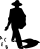
\includegraphics[width=.18\textwidth]{../plantillas/logo.png} % Insert logo in the head % {\pttitle} to insert the title at the left \hfill }
%{\hfill\textsc{\ptgroup}}
\fancyhead[R]{\hfill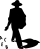
\includegraphics[width=0.7cm]{../../../img/logo.png}}
\fancyhead[L]{\textsc{\ptgroup}\hfill}
}
%\lhead{\ULCornerWallPaper{0.01}{../../img/logo.png}} % Insert logo in the head
% Group page style

\setlength{\pregroupvspace}{10em}


% Poem Title--------------------------------------------

%\renewcommand*{\pttitleenv}{flushleft} % You can change to center or flushright. Center is by default.

%	Poem title margin and indentation ----------------------

\setlength{\poemvspace}{0em} % Title margin top 
\setlength{\pttitleleftspace}{0em} % Title margin left
\setlength{\pttitlerightspace}{0em} % Title margin right

\setlength{\ptsubtitleleftspace}{0em} % Subtitle margin left
\setlength{\ptsubtitlerightspace}{0em} % Subtitle margin right

% To insert a rule in the top of the title uncomment this:
% \renewcommand*{\poemtitleformat}
% {\normalfont\bfseries%
% {\rule{10em}{0.001em}}\\*} 

\renewcommand*{\ptdefaulttitle}{} % You can change this for \renewcommand*{\ptdefaulttitle}{Untitled \textnumero\ \arabic{absoluteuntitledpoemnum}} % to set the default title

\numbertop
\renewcommand*{\titlepoemnum}{% 
\unskip\Roman{absolutepoemnum}\\} % You can change roman for arabic, and put or quit {poemnum}


% Asterism
\renewcommand{\ptspacerchar}{\bigskip\par{\large\centerline{***\medskip}}\par} % choose the character to separate the poems or stanzas, you need put \ptspacer betwen
\setcounter{ptspacernum}{1} % Number of times to repeat the spacer

% Configuration of footnote
\usepackage[bottom,flushmargin,hang,multiple]{footmisc}

% Quotes and epigraphs -------------------------------

\renewenvironment{quotation}
{\par\leftskip=1em\vskip.5\onelineskip\em}
{\par\vskip.5\onelineskip}

\renewenvironment{quote}
  {\small\list{}{\rightmargin=3.5em \leftmargin=3.5em}%
   \item\relax}
  {\endlist}

\setlength{\epigraphrule}{0em} % You can change the size of the rule

\setlength\epigraphwidth{.4\textwidth}

\renewcommand{\epigraphsize}{\footnotesize} % \epigraphsize{\small}% Default

% Spacing---------------------------------------------
% Indentation
\setlength{\parindent}{0em} % Paragraph indentation
\setlength{\ptgap}{2em} % Poem indentation. You need to insert \ptind in the poem to indent
\setlength{\parskip}{2.5ex} % Set the space inter parragraphs
\setlength{\stanzaparskip}{1em} % Set the space inter stanza
\setlength{\vindent}{3em}

% Hyphenation

\usepackage{hyphenat}
%\sloppy % suaviza las reglas de ruptura de líneas de LaTeX

 % Include the file that specifies the document structure and layout

\renewcommand{\pttitle}{Poeta en Nueva York}
\renewcommand{\ptsubtitle}{}
\renewcommand{\ptauthor}{Federico García Lorca}
\renewcommand{\ptdate}{}

% Define the dedication. 
%\renewcommand{\ptdedication}{}

\begin{document}

\newlength{\saveleftmargini} % define a temp variable for the original margin
\setlength{\saveleftmargini}{\leftmargini} % write the original margin in this variable
\setlength{\leftmargini}{0.5em} % set the left margin to zero

\thispagestyle{empty} % Suppress page numbering

%\ThisCenterWallPaper{1}{portada.jpg} % Add the background image, the first argument is the scaling - adjust this as necessary so the image fits the entire page

% \maketitle you need put the option titlepage in the \documentclass

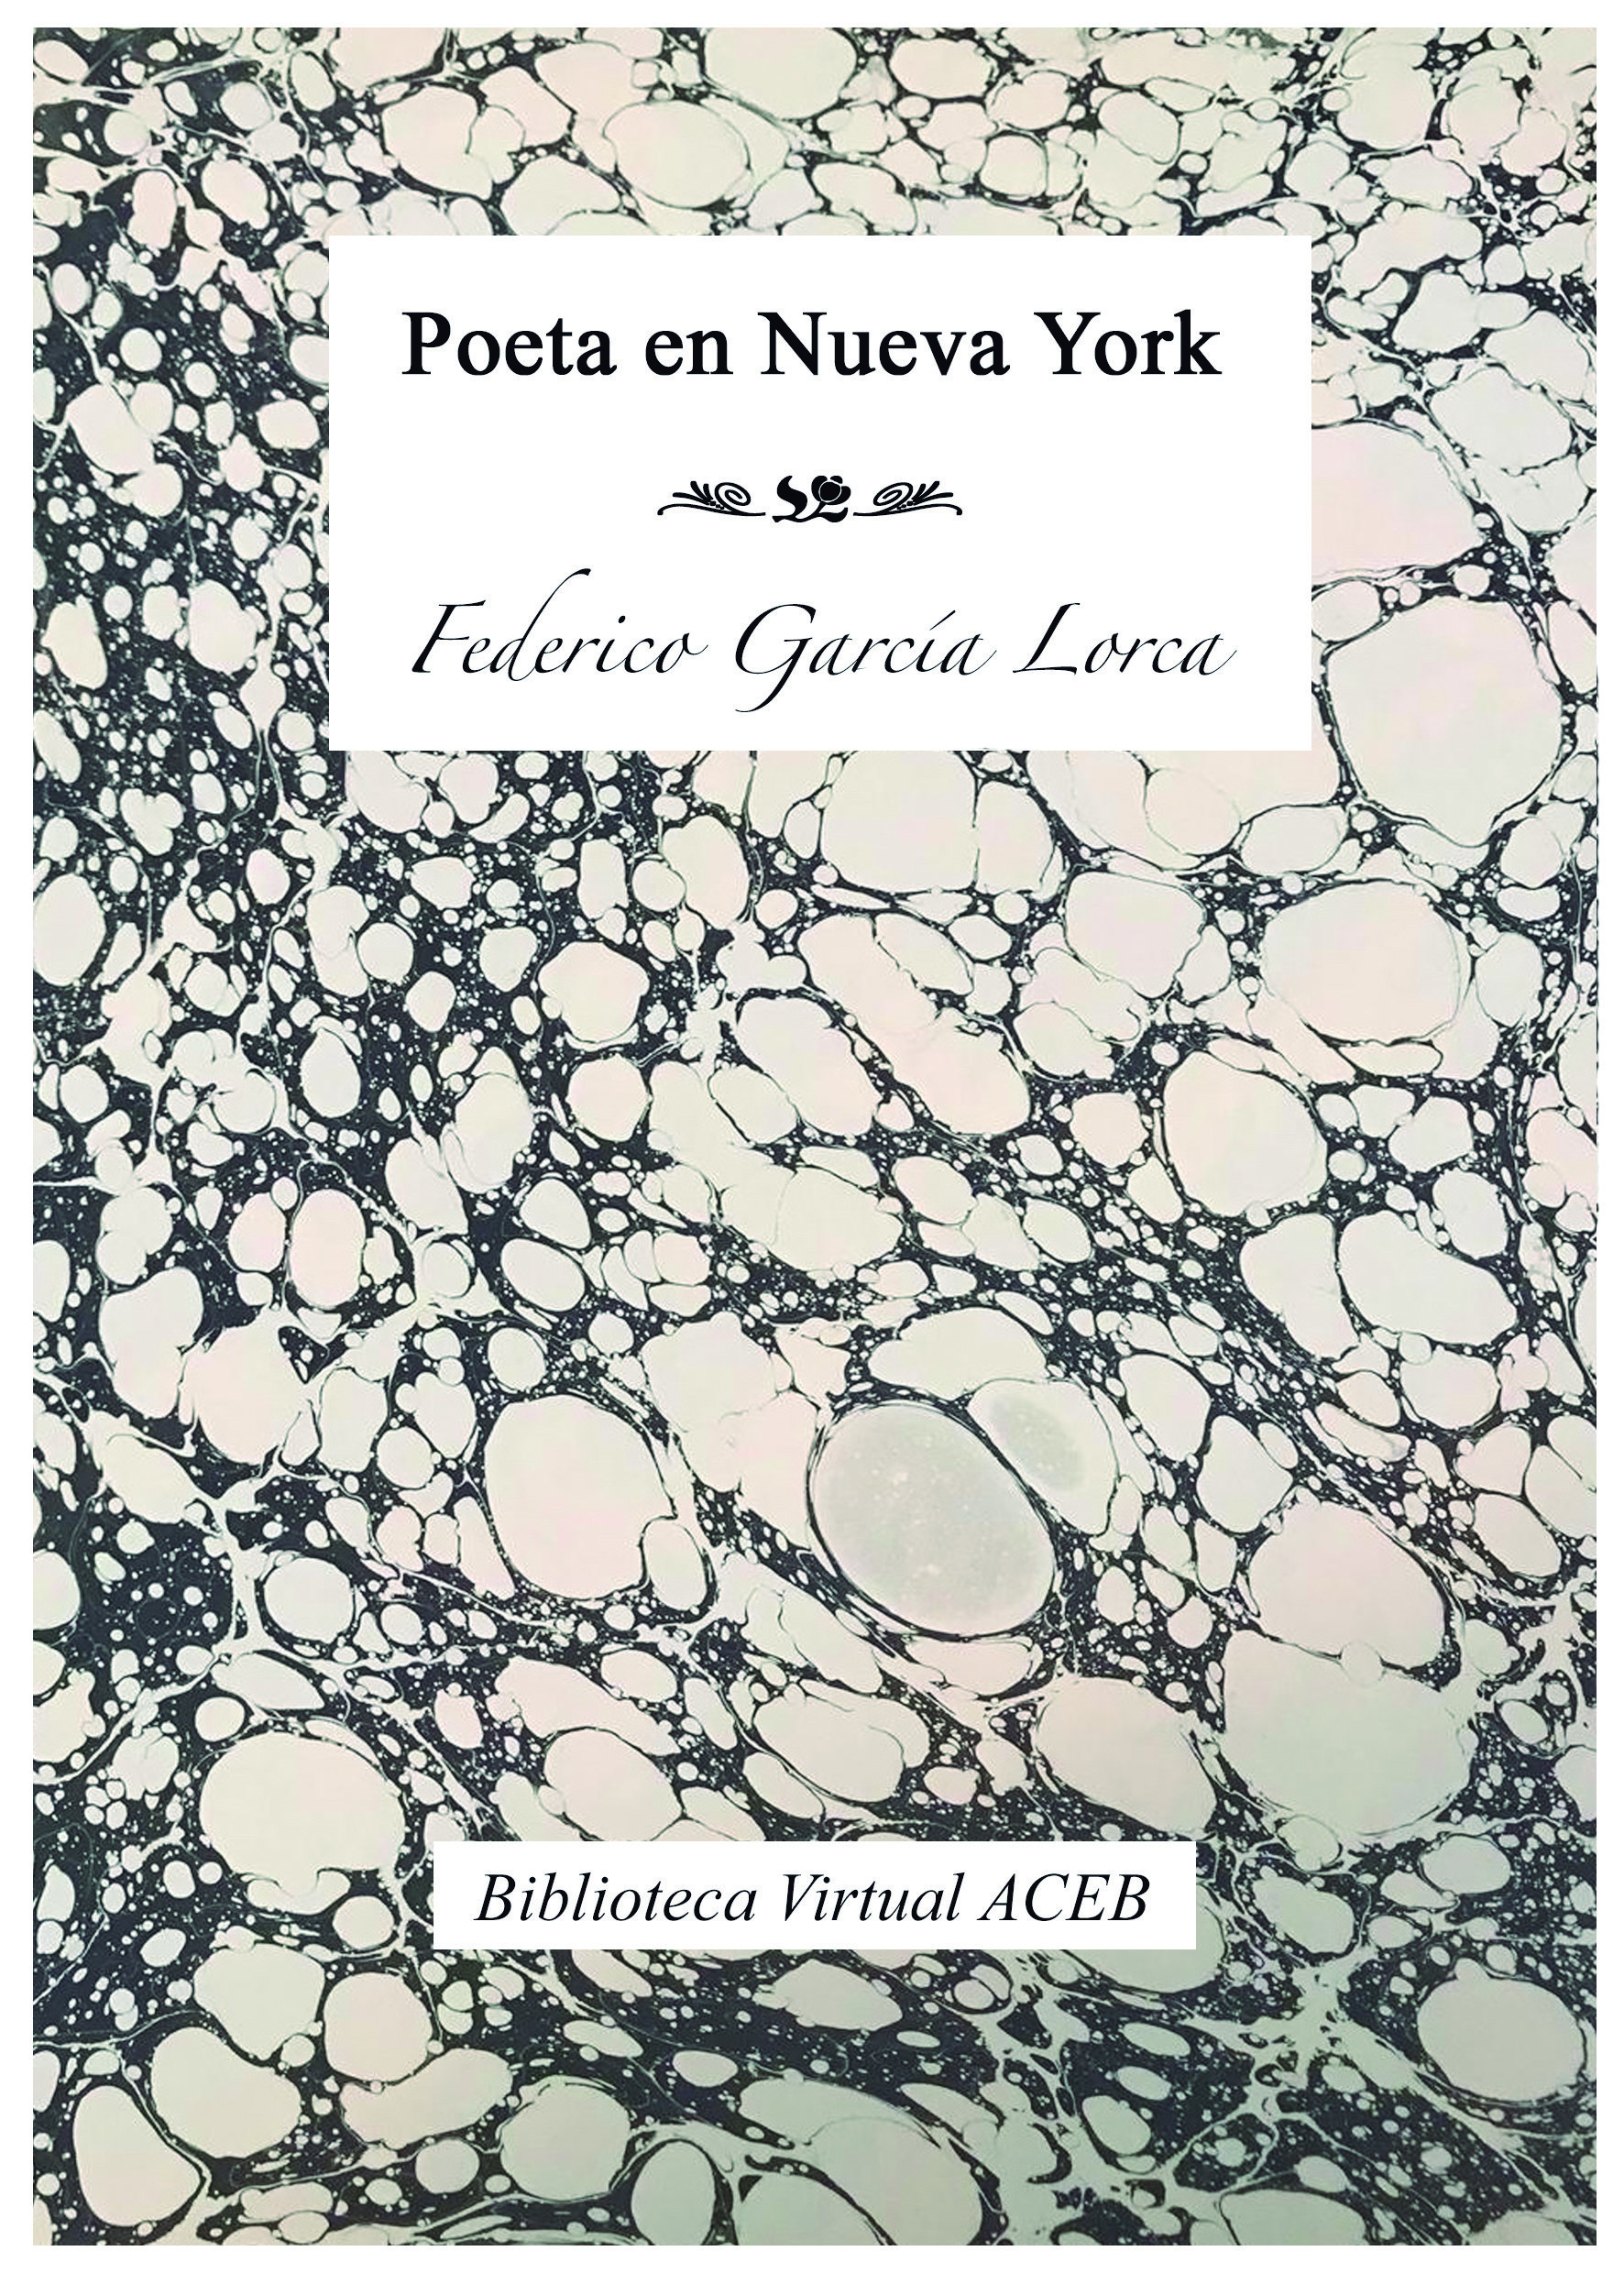
\includepdf{portada.png}
\thispagestyle{empty} % Suppress page numbering

\section*{} % Página de legal
\vspace{2em}
\begin{center}
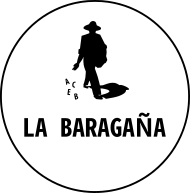
\includegraphics[width=0.25\textwidth]{../../img/granlogo.png}

\href{http://www.bibliotecavirtualaceb.org}{\textbf{Biblioteca virtual ACEB}}

\end{center}

\vfill
\copyright Federico García Lorca (del Texto)\\*\copyright Asociación Cultural La Baragaña (edición electrónica)

Esta edición por ser gratuita no precisa de ISBN o Depósito Legal. 

La versión 1.1.1 del documento ha sido finalizada el día \today. Se puede obtener una copia en distintos formatos o quizás una versión más
reciente en la página web de la asociación \href{http://www.bibliotecavirtualaceb.org/716-2}{http://www.bibliotecavirtualaceb.org/716-2}.
Para cualquier consulta puede enviar un email a: \href{mailto://contacto@bibliotecavirtualaceb.org}{contacto@bibliotecavirtualaceb.org}.

La obra está libre de restricciones conocidas de derechos de autor, pero en todo caso deben respetarse el contenido de los derechos morales de paternidad e integridad de la obra. 

El libro puede ser descargado total o parcialmente en cualquier tipo de plataforma de lectura en los siguientes términos: 
\href{https://creativecommons.org/publicdomain/mark/1.0/}{“Etiqueta de Dominio Público 1.0”}
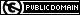
\includegraphics[scale=0.82]{../../img/public_domain.png}
\label{fig:public_domain}

\newpage

\section*{Nota del editor}

La presente edición de Poeta en Nueva York nace de la lectura y estudio
de diferentes ediciones:

\begin{itemize}

\item \emph{Poeta en Nueva York}, Colección Austral, Espasa Calpe (Segunda
edición: 31, 3, 1975).

\item \emph{Federico García Lorca. Obras completas}. RBA, Instituto Cervantes
(2005).

\item \emph{Poeta en Nueva York}. Biblioteca Virtual Miguel de Cervantes (2017).

\item \emph{Poeta en Nueva York}. Editorial Lumen, colección Palabra Menor
(Barcelona 1976.)

\end{itemize}

Este detalle, que puede parecer intrascendente al tratarse de la misma
obra, es de vital importancia pues en cada una de las citadas ediciones
aparecen cambios significativos.

Ni la edición de la Biblioteca Virtual Miguel de Cervantes ni la de
Espasa-Calpe incluyen el poema que lleva por título: \emph{Crucifixión.}
Poema que sí aparece en el capítulo VII (Vuelta a la Ciudad) en la
edición de RBA.

Los poemas: \emph{Pequeño poema infinito} y \emph{La luna pudo detenerse
al fin} aparecen en la edición de la Biblioteca Virtual Miguel de
Cervantes y en la edición de Espasa-Calpe en el capítulo X, que lleva
por título, \emph{El poeta llega a La Habana,} mientras que la edición
de RBA no los contiene dentro de Poeta en Nueva York sino en
\emph{Tierra y Luna}.

Ya en el primer poema, \emph{Vuelta de paseo}, nos encontramos en la
encrucijada de tener que elegir entre el cuarto verso de la edición de
la Biblioteca Virtual Miguel de Cervantes (refiriéndome siempre a la
edición que aparece a 7 del 11 de 2018, fecha en la que finalizamos la
presente edición) \emph{Dejaré \textbf{caer} mis cabellos,} o el cuarto
verso del mismo poema publicado por RBA, la Colección Austral de
Espasa-Calpe y otras ediciones consultadas: \emph{Dejaré \textbf{crecer}
mis cabellos.}

Otros ejemplos: En la citada edición de Espasa-Calpe y en la de la
Biblioteca Virtual Miguel de Cervantes encontramos este verso del poema
\emph{Paisaje de la multitud que orina: Fachadas de}
\textbf{crin}\emph{, de humo, anémonas, guantes de goma.} El mismo verso
en la edición de RBA: \emph{Fachadas de \textbf{orín}, de humo,
anémonas, guantes de goma.}

En el poema titulado \emph{Muerte} podemos leer: \emph{\textbf{y los
puñales} \textbf{diminutos}.} Si se trata de la edición de Espasa Calpe
o la de RBA o: \textbf{y} \textbf{\emph{los puñales}} si se trata de la
Biblioteca Virtual Miguel de Cervantes. En el poema \emph{Ciudad sin
sueño} encontramos en la edición de RBA: \emph{Las criaturas de la luna
huelen y rondan \textbf{las} cabañas}.

En las ediciones de Espasa-Calpe y Biblioteca Virtual Miguel de
Cervantes: \emph{Las criaturas de la luna huelen y rondan \textbf{sus}
cabañas.} Permítanme la broma: parece que en el periodo de tiempo
transcurrido entre la publicación de RBA y la publicación de la
Biblioteca Virtual Miguel de Cervantes, las criaturas de la luna
hubiesen comprado esas cabañas.

Según la edición que tengamos en nuestras manos: las estatuas sufren
\textbf{por} los ojos \textbf{con} la oscuridad de los ataúdes o sufren
\textbf{con} los ojos \textbf{por} la oscuridad de los ataúdes.

No me extenderé más en el tema, podría poner muchos más ejemplos, decir
que la puntuación, dependiendo de la editorial, es diferente, que lo que
para una es una coma para otra es punto o punto y coma. Que dependiendo
de la edición después de cerrar una exclamación aparece una coma, o no,
e indistintamente de si aparece o deja de aparecer, se continua con
minúscula o mayúscula sin respetar las normas de puntuación, incluso
cambiando de criterio durante una misma edición.

Como todos ustedes (supongo) no he tenido ocasión de leer el manuscrito
original de Lorca por lo que esta edición se basa en las anteriormente
mencionadas.

Estos comentarios no pretenden, en modo alguno, hacer burla del
admirable y extraordinario trabajo de las mencionadas editoriales o de
la Biblioteca Virtual Miguel de Cervantes. Si consultáramos las
ediciones en papel que sin duda poseen muchos de nuestros lectores
encontraríamos también abundantes diferencias.

Jorge Espina

\newpage

% TOC %
\maketoc

% TOP %
\renewcommand*{\topname}{Índice de poemas} % Name for the table of poems
\maketop

\nonumberpoems

\begin{hyphenrules}{nohyphenation} % Evitar la hiphenación

\epigraphhead[250]{
\emph{Furia color de amor,\\*
amor color de olvido.}\\*
\textbf{Luis Cernuda}
}
\poemgroup{Poemas de la soledad en Columbia University}


\begin{poem}{Vuelta de paseo}{}{\vspace{-1em}}

Asesinado por el cielo,\\*
entre las formas que van hacia la sierpe\\*
y las formas que buscan el cristal,\\*
dejaré crecer mis cabellos.\\!

Con el árbol de muñones que no canta\\*
y el niño con el blanco rostro de huevo.\\!

Con los animalitos de cabeza rota\\*
y el agua harapienta de los pies secos.\\!

Con todo lo que tiene cansancio sordomudo\\*
y mariposa ahogada en el tintero.\\!

Tropezando con mi rostro distinto de cada día.\\*
¡Asesinado por el cielo! \\!

\end{poem}

\begin{poem}{Intermedio}{1910}{}

Aquellos ojos míos de mil novecientos diez\\*
no vieron enterrar a los muertos,\\*
ni la feria de ceniza del que llora por la madrugada,\\*
ni el corazón que tiembla arrinconado como un caballito de mar.\\!

Aquellos ojos míos de mil novecientos diez\\*
vieron la blanca pared donde orinaban las niñas,\\*
el hocico del toro, la seta venenosa\\*
y una luna incomprensible que iluminaba por los rincones\\*
los pedazos de limón seco bajo el negro duro de las botellas.\\!

Aquellos ojos míos en el cuello de la jaca,\\*
en el seno traspasado de Santa Rosa dormida,\\*
en los tejados del amor, con gemidos y frescas manos,\\*
en un jardín donde los gatos se comían a las ranas.\\!

Desván donde el polvo viejo congrega estatuas y musgos,\\*
cajas que guardan silencio de cangrejos devorados\\*
en el sitio donde el sueño tropezaba con su realidad.\\*
Allí mis pequeños ojos.\\!

No preguntarme nada. He visto que las cosas\\*
cuando buscan su curso encuentran su vacío.\\*
Hay un dolor de huecos por el aire sin gente\\*
y en mis ojos criaturas vestidas ¡sin desnudo! \\!

\end{poem}

\begin{poem}{Fábula y rueda de los tres amigos}{}{}

Enrique,\\*
Emilio,\\*
Lorenzo.\\!

Estaban los tres helados:\\*
Enrique por el mundo de las camas;\\*
Emilio por el mundo de los ojos y las heridas de las manos,\\*
Lorenzo por el mundo de las universidades sin tejados.\\!

Lorenzo,\\*
Emilio,\\*
Enrique.\\!

Estaban los tres quemados:\\*
Lorenzo por el mundo de las hojas y las bolas de billar;\\*
Emilio por el mundo de la sangre y los alfileres blancos,\\*
Enrique por el mundo de los muertos y los periódicos abandonados.\\!

Lorenzo,\\*
Emilio,\\*
Enrique.\\!

Estaban los tres enterrados.\\*
Lorenzo en un seno de Flora;\\*
Emilio en la yerta ginebra que se olvida en el vaso,\\*
Enrique en la hormiga, en el mar y en los ojos vacíos de los pájaros.\\!

Lorenzo,\\*
Emilio,\\*
Enrique.\\!

Fueron los tres en mis manos\\*
tres montañas chinas,\\*
tres sombras de caballo,\\*
tres paisajes de nieve y una cabaña de azucenas\\*
por los palomares donde la luna se pone plana bajo el gallo.\\!

Uno\\*
y uno\\*
y uno.\\!

Estaban los tres momificados.\\*
Con las moscas del invierno,\\*
con los tinteros que orina el perro y desprecia el vilano,\\*
con la brisa que hiela el corazón de todas las madres,\\*
por los blancos derribos de Júpiter donde meriendan muerte\\*
los borrachos.\\!

Tres\\*
y dos\\*
y uno.\\!

Los vi perderse llorando y cantando\\*
por un huevo de gallina,\\*
por la noche que enseñaba su esqueleto de tabaco,\\*
por mi dolor lleno de rostros y punzantes esquirlas de luna,\\*
por mi alegría de ruedas dentadas y látigos,\\

por mi pecho turbado por las palomas,\\*
por mi muerte desierta con un solo paseante equivocado.\\!

Yo había matado la quinta luna\\*
y bebían agua por las fuentes los abanicos y los aplausos.\\*
Tibia leche encerrada de las recién paridas\\*
agitaba las rosas con un largo dolor blanco.\\!

Enrique,\\*
Emilio,\\*
Lorenzo.\\!

Diana es dura,\\*
pero a veces tiene los pechos nublados.\\*
Puede la piedra blanca latir en la sangre del ciervo\\*
y el ciervo puede soñar por los ojos de un caballo.\\*
Cuando se hundieron las formas puras\\*
bajo el cri cri de las margaritas,\\*
comprendí que me habían asesinado.\\*
Recorrieron los cafés y los cementerios y las iglesias,\\*
abrieron los toneles y los armarios,\\*
destrozaron tres esqueletos para arrancar sus dientes de oro.\\*
Ya no me encontraron.\\*
¿No me encontraron?\\*
No. No me encontraron.\\*
Pero se supo que la sexta luna huyó torrente arriba,\\*
y que el mar recordó ¡de pronto!\\*
los nombres de todos sus ahogados.\\!

\end{poem}

\begin{poem}{Tu infancia en Menton}{}{}

\epigraph{
\emph{\hspace{-1.5em}Sí, tu niñez: ya fábula de fuentes.}\\*
\hspace{-1.5em}\textbf{Jorge Guillén}
}

Sí, tu niñez ya fábula de fuentes.\\*
El tren y la mujer que llena el cielo.\\*
Tu soledad esquiva en los hoteles\\*
y tu máscara pura de otro signo.\\*
Es la niñez del mar y tu silencio\\*
donde los sabios vidrios se quebraban.\\*
Es tu yerta ignorancia donde estuvo\\*
mi torso limitado por el fuego.\\*
Norma de amor te di, hombre de Apolo,\\*
llanto con ruiseñor enajenado,\\*
pero, pasto de ruina, te afilabas\\*
para los breves sueños indecisos.\\*
Pensamiento de enfrente, luz de ayer,\\*
índices y señales del acaso.\\*
Tu cintura de arena sin sosiego\\*
atiende sólo rastros que no escalan.\\*
Pero yo he de buscar por los rincones\\*
tu alma tibia sin ti que no te entiende,\\*
con el dolor de Apolo detenido\\*
con que he roto la máscara que llevas.\\*
Allí, león, allí, furia del cielo,\\

te dejaré pacer en mis mejillas;\\*
allí, caballo azul de mi locura,\\*
pulso de nebulosa y minutero,\\*
he de buscar las piedras de alacranes\\*
y los vestidos de tu madre niña,\\*
llanto de medianoche y paño roto\\*
que quitó luna de la sien del muerto.\\*
Sí, tu niñez ya fábula de fuentes.\\*
Alma extraña de mi hueco de venas,\\*
te he de buscar pequeña y sin raíces.\\*
¡Amor de siempre, amor, amor de nunca!\\

¡Oh, sí! Yo quiero. ¡Amor, amor! Dejadme.\\*
No me tapen la boca los que buscan\\*
espigas de Saturno por la nieve\\*
o castran animales por un cielo,\\*
clínica y selva de la anatomía.\\*
Amor, amor, amor. Niñez del mar.\\*
Tu alma tibia sin ti que no te entiende.\\*
Amor, amor, un vuelo de la corza\\*
por el pecho sin fin de la blancura.\\*
Y tu niñez, amor, y tu niñez.\\*
El tren y la mujer que llena el cielo.\\*
Ni tú, ni yo, ni el aire, ni las hojas.\\*
Sí, tu niñez ya fábula de fuentes.\\!

\end{poem}

\epigraphhead[250]{

\emph{Para Ángel del Río}

}


\poemgroup{Los negros}

\begin{poem}{Norma y paraíso de los negros}{}{\vspace{-1em}}

Odian la sombra del pájaro\\*
sobre el pleamar de la blanca mejilla\\*
y el conflicto de luz y viento\\*
en el salón de la nieve fría.\\!

Odian la flecha sin cuerpo,\\*
el pañuelo exacto de la despedida,\\*
la aguja que mantiene presión y rosa\\*
en el gramíneo rubor de la sonrisa.\\!

Aman el azul desierto,\\*
las vacilantes expresiones bovinas,\\*
la mentirosa luna de los polos,\\*
la danza curva del agua en la orilla.\\!

Con la ciencia del tronco y del rastro\\*
llenan de nervios luminosos la arcilla\\*
y patinan lúbricos por agua y arenas\\*
gustando la amarga frescura de su milenaria saliva.\\!

Es por el azul crujiente,\\*
azul sin un gusano ni una huella dormida,\\*
donde los huevos de avestruz quedan eternos\\*
y deambulan intactas las lluvias bailarinas.\\!

Es por el azul sin historia,\\*
azul de una noche sin temor de día,\\*
azul donde el desnudo del viento va quebrando\\*
los camellos sonámbulos de las nubes vacías.\\*
Es allí donde sueñan los torsos bajo la gula de la hierba.\\*
Allí los corales empapan la desesperación de la tinta,\\*
los durmientes borran sus perfiles bajo la madeja de los caracoles\\*
y queda el hueco de la danza sobre las últimas cenizas.\\!

\end{poem}

\begin{poem}{El rey del Harlem}{}{\vspace{-1em}}

Con una cuchara\\*
arrancaba los ojos a los cocodrilos\\*
y golpeaba el trasero de los monos.\\*
Con una cuchara.\\!

Fuego de siempre dormía en los pedernales\\*
y los escarabajos borrachos de anís\\*
olvidaban el musgo de las aldeas.\\!

Aquel viejo cubierto de setas\\*
iba al sitio donde lloraban los negros\\*
mientras crujía la cuchara del rey\\*
y llegaban los tanques de agua podrida.\\!

Las rosas huían por los filos\\*
de las últimas curvas del aire,\\*
y en los montones de azafrán\\*
los niños machacaban pequeñas ardillas\\*
con un rubor de frenesí manchado.\\!

Es preciso cruzar los puentes\\*
y llegar al rubor negro\\*
para que el perfume de pulmón\\*
nos golpee las sienes con su vestido\\*
de caliente piña.\\!

Es preciso matar al rubio vendedor de aguardiente,\\*
a todos los amigos de la manzana y de la arena,\\*
y es necesario dar con los puños cerrados\\*
a las pequeñas judías que tiemblan llenas de burbujas,\\*
para que el rey de Harlem cante con su muchedumbre,\\*
para que los cocodrilos duerman en largas filas\\*
bajo el amianto de la luna,\\*
y para que nadie dude de la infinita belleza\\*
de los plumeros, los ralladores, los cobres y las cacerolas de las cocinas.\\!

¡Ay Harlem! ¡Ay Harlem! ¡Ay Harlem!\\*
No hay angustia comparable a tus rojos oprimidos,\\*
a tu sangre estremecida dentro del eclipse oscuro,\\*
a tu violencia granate sordomuda en la penumbra,\\*
a tu gran rey prisionero, con un traje de conserje.\\!

\ptspacer

Tenía la noche una hendidura y quietas salamandras de marfil.\\*
Las muchachas americanas\\*
llevaban niños y monedas en el vientre\\*
y los muchachos se desmayaban en la cruz del desperezo.\\!

Ellos son.\\*
Ellos son los que beben el whisky de plata junto a los volcanes y\\*
tragan pedacitos de corazón por las heladas montañas del oso.\\!

Aquella noche el rey de Harlem con una durísima cuchara\\*
arrancaba los ojos a los cocodrilos\\*
y golpeaba el trasero de los monos.\\*
Con una cuchara.\\*
Los negros lloraban confundidos\\*
entre paraguas y soles de oro,\\*
los mulatos estiraban gomas, ansiosos de llegar al torso blanco,\\*
y el viento empañaba espejos\\*
y quebraba las venas de los bailarines.\\!

Negros, Negros, Negros, Negros.\\*
La sangre no tiene puertas en vuestra noche boca arriba.\\*
No hay rubor. Sangre furiosa por debajo de las pieles,\\*
viva en la espina del puñal y en el pecho de los paisajes, bajo las\\*
pinzas y las retamas de la celeste luna de Cáncer.\\!

Sangre que busca por mil caminos muertes enharinadas y ceniza de nardo,\\*
cielos yertos, en declive, donde las colonias de planetas\\*
rueden por las playas con los objetos abandonados.\\!

Sangre que mira lenta con el rabo del ojo,\\*
hecha de espartos exprimidos, néctares de subterráneos.\\*
Sangre que oxida el alisio descuidado en una huella\\*
y disuelve a las mariposas en los cristales de la ventana.\\!

Es la sangre que viene, que vendrá\\*
por los tejados y azoteas, por todas partes,\\*
para quemar la clorofila de las mujeres rubias,\\*
para gemir al pie de las camas ante el insomnio de los lavabos\\*
y estrellarse en una aurora de tabaco y bajo amarillo.\\!

Hay que huir,\\*
huir por las esquinas y encerrarse en los últimos pisos,\\*
porque el tuétano del bosque penetrará por las rendijas\\*
para dejar en vuestra carne una leve huella de eclipse\\*
y una falsa tristeza de guante desteñido y rosa química.\\!

\ptspacer

Es por el silencio sapientísimo\\*
cuando los camareros y los cocineros y los que limpian con la lengua\\*
las heridas de los millonarios\\*
buscan al rey por las calles o en los ángulos del salitre.\\!

Un viento sur de madera, oblicuo en el negro fango,\\*
escupe a las barcas rotas y se clava puntillas en los hombros; un\\*
viento sur que lleva\\*
colmillos, girasoles, alfabetos\\*
y una pila de Volta con avispas ahogadas.\\!

El olvido estaba expresado por tres gotas de tinta sobre el monóculo.\\*
El amor, por un solo rostro invisible a flor de piedra.\\*
Médulas y corolas componían sobre las nubes\\*
un desierto de tallos sin una sola rosa.\\!

\newpage

\ptspacer

A la izquierda, a la derecha, por el Sur y por el Norte,\\*
se levanta el muro impasible\\*
para el topo, la aguja del agua.\\*
No busquéis, negros, su grieta\\*
para hallar la máscara infinita.\\*
Buscad el gran sol del centro\\*
hechos una piña zumbadora.\\*
El sol que se desliza por los bosques\\*
seguro de no encontrar una ninfa,\\*
el sol que destruye números y no ha cruzado nunca un sueño,\\*
el tatuado sol que baja por el río\\*
y muge seguido de caimanes.\\!

Negros, Negros, Negros, Negros.\\*
Jamás sierpe, ni cebra, ni mula\\*
palidecieron al morir.\\*
El leñador no sabe cuándo expiran\\*
los clamorosos árboles que corta.\\*
Aguardad bajo la sombra vegetal de vuestro rey\\*
a que cicutas .y cardos y ortigas turben postreras azoteas.\\!

Entonces, negros, entonces, entonces,\\*
podréis besar con frenesí las ruedas de las bicicletas,\\*
poner parejas de microscopios en las cuevas de las ardillas\\*
y danzar al fin, sin duda, mientras las flores erizadas\\*
asesinan a nuestro Moisés casi en los juncos del cielo.\\!

¡Ay, Harlem disfrazada!\\*
¡Ay, Harlem, amenazada por un gentío de trajes sin cabeza!\\*
Me llega tu rumor,\\*
me llega tu rumor atravesando troncos y ascensores,\\*
a través de láminas grises\\*
donde flotan tus automóviles cubiertos de dientes,\\*
a través de los caballos muertos y los crímenes diminutos,\\*
a través de tu gran rey desesperado\\*
cuyas barbas llegan al mar.\\!

\end{poem}

\begin{poem}{Iglesia Abandonada}{Balada de la Gran Guerra}{}

Yo tenía un hijo que se llamaba Juan.\\*
Yo tenía un hijo.\\*
Se perdió por los arcos un viernes de todos los muertos.\\*
Le vi jugar en las últimas escaleras de la misa\\*
y echaba un cubito de hojalata en el corazón del sacerdote.\\*
He golpeado los ataúdes. ¡Mi hijo! ¡Mi hijo! ¡Mi hijo!\\*
Saqué una pata de gallina por detrás de la luna y luego\\*
comprendí que mi niña era un pez\\*
por donde se alejan las carretas.\\*
Yo tenía una niña.\\*
Yo tenía un pez muerto bajo la ceniza de los incensarios.\\*
Yo tenía un mar. ¿De qué? ¡Dios mío! ¡Un mar!\\*
Subí a tocar las campanas, pero las frutas tenían gusanos.\\*
y las cerillas apagadas\\*
se comían los trigos de la primavera.\\*
Yo vi la transparente cigüeña de alcohol\\*
mondar las negras cabezas de los soldados agonizantes\\*
y vi las cabañas de goma\\*
donde giraban las copas llenas de lágrimas.\\*
En las anémonas del ofertorio te encontraré, ¡corazón mío!,\\*
cuando el sacerdote levante la mula y el buey con sus fuertes brazos,\\*
para espantar los sapos nocturnos que rondan los helados paisajes del
cáliz.\\*
Yo tenía un hijo que era un gigante,\\

pero los muertos son más fuertes y saben devorar pedazos de cielo.\\*
Si mi niño hubiera sido un oso,\\*
yo no temería el sigilo de los caimanes,\\*
ni hubiese visto el mar amarrado a los árboles\\*
para ser fornicado y herido por el tropel de los regimientos.\\*
¡Si mi niño hubiera sido un oso!\\*
Me envolveré sobre esta lona dura para no sentir el frío de los
musgos.\\*
Sé muy bien que me darán una manga o la corbata;\\*
pero en el centro de la misa yo romperé el timón y entonces\\*
vendrá a la piedra la locura de pingüinos y gaviotas\\*
que harán decir a los que duermen y a los que cantan por las esquinas:\\*
Él tenía un hijo.\\*
¡Un hijo! ¡Un hijo! ¡Un hijo\\*
que no era más que suyo porque era su hijo!\\*
¡Su hijo! ¡Su hijo! ¡Su hijo! \\!

\end{poem}



\epigraphhead[250]{

\hspace{-1.5em}\emph{A Rafael R. Rapún}
\vspace{5em}

\hspace{-1.5em}\emph{Un pájaro de papel en el pecho}\\*
\emph{dice que el tiempo de los huesos no ha llegado.}\\*
\textbf{Vicente Aleixandre}
}
\poemgroup{Calles y sueños}{}{\vspace{-1em}}

\begin{poem}{Danza de la muerte}{}{\vspace{-1em}}

\emph{El mascarón. ¡Mirad el mascarón!\\*
¡Cómo viene del África a New York!}\\!

Se fueron los árboles de la pimienta,\\*
los pequeños botones de fósforo.\\*
Se fueron los camellos de carne desgarrada\\*
y los valles de luz que el cisne levantaba con el pico.\\!

Era el momento de las cosas secas,\\*
de la espiga en el ojo y el gato laminado,\\*
del óxido de hierro de los grandes puentes\\*
y el definitivo silencio del corcho.\\!

Era la gran reunión de los animales muertos,\\*
traspasados por las espadas de la luz;\\*
la alegría eterna del hipopótamo con las pezuñas de ceniza\\*
y de la gacela con una siempreviva en la garganta.\\!

En la marchita soledad sin honda\\*
el abollado mascarón danzaba.\\*
Medio lado del mundo era de arena,\\*
mercurio y sol dormido el otro medio.\\!

\emph{El mascarón. ¡Mirad el mascarón!\\*
!Arena, caimán y miedo sobre Nueva York!} \\!

Desfiladeros de cal aprisionaban un cielo vacío\\*
donde sonaban las voces de los que mueren bajo el guano.\\*
Un cielo mondado y puro, idéntico a sí mismo,\\*
con el bozo y lirio agudo de sus montañas invisibles, \\!

acabó con los más leves tallitos del canto\\*
y se fue al diluvio empaquetado de la savia,\\*
a través del descanso de los últimos desfiles,\\*
levantando con el rabo pedazos de espejo.\\!

Cuando el chino lloraba en el tejado\\*
sin encontrar el desnudo de su mujer\\*
y el director del banco observando el manómetro\\*
que mide el cruel silencio de la moneda,\\*
el mascarón llegaba a Wall Street.\\!

No es extraño para la danza\\*
este columbario que pone los ojos amarillos.\\*
De la esfinge a la caja de caudales hay un hilo tenso\\*
que atraviesa el corazón de todos los niños pobres.\\*
El ímpetu primitivo baila con el ímpetu mecánico,\\*
ignorantes en su frenesí de la luz original.\\*
Porque si la rueda olvida su fórmula,\\*
ya puede cantar desnuda con las manadas de caballos:\\*
y si una llama quema los helados proyectos,\\*
el cielo tendrá que huir ante el tumulto de las ventanas.\\!

No es extraño este sitio para la danza, yo lo digo.\\*
El mascarón bailará entre columnas de sangre y de números,\\*
entre huracanes de oro y gemidos de obreros parados\\*
que aullarán, noche oscura, por tu tiempo sin luces,\\*
¡oh salvaje Norteamérica!, ¡oh impúdica!, ¡oh salvaje,\\*
tendida en la frontera de la nieve! \\!

\emph{El mascarón. ¡Mirad el mascarón!\\*
¡Qué ola de fango y luciérnaga sobre Nueva York!} \\!

Yo estaba en la terraza luchando con la luna.\\*
Enjambres de ventanas acribillaban un muslo de la noche.\\*
En mis ojos bebían las dulces vacas de los cielos.\\*
Y las brisas de largos remos\\*
golpeaban los cenicientos cristales de Broadway.\\!

La gota de sangre buscaba la luz de la yema del astro\\*
para fingir una muerta semilla de manzana.\\*
El aire de la llanura, empujado por los pastores,\\*
temblaba con un miedo de molusco sin concha.\\!

Pero no son los muertos los que bailan,\\*
estoy seguro.\\*
Los muertos están embebidos, devorando sus propias manos.\\*
Son los otros los que bailan con el mascarón y su vihuela;\\*
son los otros, los borrachos de plata, los hombres fríos, \\!

los que crecen en el cruce de los muslos y llamas duras,\\*
los que buscan la lombriz en el paisaje de las escaleras,\\*
los que beben en el banco lágrimas de niña muerta\\*
o los que comen por las esquinas diminutas pirámides del alba.\\!

¡Que no baile el Papa!\\*
¡No, que no baile el Papa!\\*
Ni el Rey,\\*
ni el millonario de dientes azules,\\*
ni las bailarinas secas de las catedrales,\\*
ni constructores, ni esmeraldas, ni locos, ni sodomitas.\\*
Sólo este mascarón,\\*
este mascarón de vieja escarlatina,\\*
¡sólo este mascarón! \\!

Que ya las cobras silbarán por los últimos pisos,\\*
que ya las ortigas estremecerán patios y terrazas,\\*
que ya la Bolsa será una pirámide de musgo,\\*
que ya vendrán lianas después de los fusiles\\*
y muy pronto, muy pronto, muy pronto.\\*
¡Ay, Wall Street! \\!

\emph{El mascarón. ¡Mirad el mascarón!\\*
¡Cómo escupe veneno de bosque\\*
por la angustia imperfecta de Nueva York!} \\!

\end{poem}

\begin{poem}{Paisaje de la multitud que vomita}{Anochecer de Coney Island \footnote{New York, 29 de diciembre de 1929}}{}

La mujer gorda venía delante\\*
arrancando las raíces y mojando el pergamino de los tambores:\\*
la mujer gorda\\*
que vuelve del revés los pulpos agonizantes.\\*
La mujer gorda, enemiga de la luna,\\*
corría por las calles y los pisos deshabitados\\*
y dejaba por los rincones pequeñas calaveras de paloma\\*
y levantaba las furias de los banquetes de los siglos últimos\\*
y llamaba al demonio del pan por las colinas del cielo barrido y\\*
filtraba un ansia de luz en las circulaciones subterráneas.\\*
Son los cementerios, lo sé, son los cementerios\\*
y el dolor de las cocinas enterradas bajo la arena,\\*
son los muertos, los faisanes y las manzanas de otra hora los\\*
que nos empujan en la garganta.\\!

Llegaban los rumores de la selva del vómito\\*
con las mujeres vacías, con niños de cera caliente,\\*
con árboles fermentados y camareros incansables\\*
que sirven platos de sal bajo las arpas de la saliva.\\*
Sin remedio, hijo mío, ¡vomita! No hay remedio.\\*
No es el vómito de los húsares sobre los pechos de la prostituta,\\*
ni el vómito del gato que se tragó una rana por descuido.\\*
Son los muertos que arañan con sus manos de tierra\\*
las puertas de pedernal donde se pudren nublos y postres.\\!

La mujer gorda venía delante\\*
con las gentes de los barcos, de las tabernas y de los jardines.\\*
El vómito agitaba delicadamente sus tambores\\*
entre algunas niñas de sangre\\*
que pedían protección a la luna.\\*
¡Ay de mí! ¡Ay de mí! ¡Ay de mí!\\*
Esta mirada mía fue mía, pero ya no es mía,\\*
esta mirada que tiembla desnuda por el alcohol\\*
y despide barcos increíbles\\*
por las anémonas de los muelles.\\*
Me defiendo con esta mirada\\*
que mana de las ondas por donde el alba no se atreve,\\*
yo, poeta sin brazos, perdido\\*
entre la multitud que vomita,\\*
sin caballo efusivo que corte\\*
los espesos musgos de mis sienes.\\*
Pero la mujer gorda seguía delante\\*
y la gente buscaba las farmacias\\*
donde el amargo trópico se fija.\\*
Sólo cuando izaron la bandera y llegaron los primeros canes\\*
la ciudad entera se agolpó en las barandillas del embarcadero.\\!

\end{poem}

\begin{poem}{Paisaje de la multitud que orina}{Nocturno de Battery Place}{}

Se quedaron solos:\\*
aguardaban la velocidad de las últimas bicicletas.\\*
Se quedaron solas:\\*
esperaban la muerte de un niño en el velero japonés.\\*
Se quedaron solos y solas,\\*
soñando con los picos abiertos de los pájaros agonizantes\\*
con el agudo quitasol que pincha\\*
al sapo recién aplastado,\\*
bajo un silencio con mil orejas\\*
y diminutas bocas de agua\\*
en los desfiladeros que resisten\\*
el ataque violento de la luna.\\*
Lloraba el niño del velero y se quebraban los corazones\\*
angustiados por el testigo y la vigilia de todas las cosas\\*
y porque todavía en el suelo celeste de negras huellas\\*
gritaban nombres oscuros, salivas y radios de níquel.\\*
No importa que el niño calle cuando le clavan el último alfiler,\\*
no importa la derrota de la brisa en la corola del algodón,\\*
porque hay un mundo de la muerte con marineros definitivos\\*
que se asomarán a los arcos y os helarán por detrás de los árboles.\\*
Es inútil buscar el recodo\\*
donde la noche olvida su viaje\\*
y acechar un silencio que no tenga\\*
trajes rotos y cáscaras y llanto,\\*
porque tan sólo el diminuto banquete de la araña\\*
basta para romper el equilibrio de todo el cielo.\\
No hay remedio para el gemido del velero japonés,\\
ni para estas gentes ocultas que tropiezan con las esquinas.\\
El campo se muerde la cola para unir las raíces en un punto\\
y el ovillo busca por la grama su ansia de longitud insatisfecha.\\
¡La luna! Los policías. ¡Las sirenas de los transatlánticos! \\*
Fachadas de crin, de humo, anémonas, guantes de goma.\\*
Todo está roto por la noche,\\*
abierta de piernas sobre las terrazas.\\*
Todo está roto por los tibios caños\\*
de una terrible fuente silenciosa.\\*
¡Oh gentes! ¡Oh mujercillas! ¡Oh soldados!\\*
Será preciso viajar por los ojos de los idiotas,\\*
campos libres donde silban mansas cobras deslumbradas,\\*
paisajes llenos de sepulcros que producen fresquísimas manzanas,\\*
\vspace{-1em}para que venga la luz desmedida\\*
que temen los ricos detrás de sus lupas,\\*
el olor de un solo cuerpo con la doble vertiente de lis y rata\\*
y para que se quemen estas gentes que pueden orinar alrededor de un gemido\\*
o en los cristales donde se comprenden las olas nunca repetidas.\\!

\end{poem}

\begin{poem}{Asesinato}{Dos voces de madrugada en Riverside Drive}{}

-\emph{¿Cómo fue?}\\*
-Una grieta en la mejilla.\\*
¡Eso es todo!\\*
Una uña que aprieta el tallo.\\*
Un alfiler que bucea\\*
hasta encontrar las raicillas del grito.\\*
Y el mar deja de moverse.\\*
\emph{-¿Cómo, cómo fue? }\\*
-Así\\*
\emph{-¡Déjame! ¿De esa manera? }\\*
Sí.\\*
El corazón salió solo.\\*
\emph{-¡Ay, ay de mí!} \\!

\end{poem}

\begin{poem}{Navidad en el Hudson}{\footnote{New York, 27 de diciembre de 1929}}{\vspace{-1em}}

¡Esa esponja gris!\\*
Ese marinero recién degollado.\\*
Ese río grande.\\*
Esa brisa de límites oscuros.\\*
Ese filo, amor, ese filo.\\*
Estaban los cuatro marineros luchando con el mundo.\\*
con el mundo de aristas que ven todos los ojos,\\*
con el mundo que no se puede recorrer sin caballos.\\*
Estaban uno, cien, mil marineros\\*
luchando con el mundo de las agudas velocidades,\\*
sin enterarse de que el mundo\\*
estaba solo por el cielo.\\!

El mundo solo por el cielo solo.\\*
Son las colinas de martillos y el triunfo de la hierba espesa.\\*
Son los vivísimos hormigueros y las monedas en el fango.\\*
El mundo solo por el cielo solo\\*
y el aire a la salida de todas las aldeas.\\*
Cantaba la lombriz el terror de la rueda\\*
y el marinero degollado\\*
cantaba al oso de agua que lo había de estrechar;\\*
y todos cantaban aleluya,\\*
aleluya. Cielo desierto.\\*
Es lo mismo, ¡lo mismo!, aleluya.\\!

He pasado toda la noche en los andamios de los arrabales\\*
dejándome la sangre por la escayola de los proyectos,\\*
ayudando a los marineros a recoger las velas desgarradas.\\*
Y estoy con las manos vacías en el rumor de la desembocadura.\\*
No importa que cada minuto\\*
un niño nuevo agite sus ramitos de venas,\\*
ni que el parto de la víbora, desatado bajo las ramas,\\*
calme la sed de sangre de los que miran el desnudo.\\*
Lo que importa es esto: hueco. Mundo solo. Desembocadura.\\*
Alba no. Fábula inerte.\\*
Sólo esto: desembocadura.\\*
¡Oh esponja mía gris!\\*
¡Oh cuello mío recién degollado!\\*
¡Oh río grande mío!\\*
¡Oh brisa mía de límites que no son míos!\\*
¡Oh filo de mi amor, oh hiriente filo! \\!

\end{poem}

\begin{poem}{Ciudad sin sueño}{Nocturno de Brooklyn Bridge}{}

No duerme nadie por el cielo. Nadie, nadie.\\*
No duerme nadie.\\*
Las criaturas de la luna huelen y rondan sus cabañas.\\*
Vendrán las iguanas vivas a morder a los hombres que no sueñan\\*
y el que huye con el corazón roto encontrará por las esquinas\\*
al increíble cocodrilo quieto bajo la tierna protesta de los astros.\\!

No duerme nadie por el mundo. Nadie, nadie.\\*
No duerme nadie.\\*
Hay un muerto en el cementerio más lejano\\*
que se queja tres años\\*
porque tiene un paisaje seco en la rodilla\\*
y el niño que enterraron esta mañana lloraba tanto\\*
que hubo necesidad de llamar a los perros para que callase.\\!

No es sueño la vida. ¡Alerta! ¡Alerta! ¡Alerta!\\*
Nos caemos por las escaleras para comer la tierra húmeda\\*
o subimos al filo de la nieve con el coro de las dalias muertas.\\*
Pero no hay olvido, ni sueño:\\*
carne viva. Los besos atan las bocas\\*
en una maraña de venas recientes\\*
y al que le duele su dolor le dolerá sin descanso\\*
y al que teme la muerte la llevará sobre sus hombros.\\!

Un día\\*
los caballos vivirán en las tabernas\\*
y las hormigas furiosas\\

atacarán los cielos amarillos que se refugian en los ojos de las vacas.\\!

Otro día\\*
veremos la resurrección de las mariposas disecadas\\*
y aun andando por un paisaje de esponjas grises y barcos mudos\\*
veremos brillar nuestro anillo y manar rosas de nuestra lengua.\\*
¡Alerta! ¡Alerta! ¡Alerta\\*
a los que guardan todavía huellas de zarpa y aguacero!\\*
Aquel muchacho que llora porque no sabe la invención del puente\\*
o a aquel muerto que ya no tiene más que la cabeza y un zapato,\\*
hay que llevarlos al muro donde iguanas y sierpes esperan,\\*
donde espera la dentadura del oso,\\*
donde espera la mano momificada del niño\\*
y la piel del camello se eriza con un violento escalofrío azul.\\!

No duerme nadie por el cielo. Nadie, nadie.\\*
No duerme nadie.\\*
Pero si alguien cierra los ojos,\\*
¡azotadlo, hijos míos, azotadlo!\\*
Haya un panorama de ojos abiertos\\*
y amargas llagas encendidas.\\*
No duerme nadie por el mundo. Nadie, nadie.\\*
Ya lo he dicho.\\*
No duerme nadie.\\*
Pero si alguien tiene por la noche exceso de musgo en las sienes,\\*
abrid los escotillones para que vea bajo la luna\\*
las copas falsas, el veneno y la calavera de los teatros.\\!

\end{poem}

\begin{poem}{Panorama ciego de Nueva York}{}{}

Si no son los pájaros\\*
cubiertos de ceniza,\\*
si no son los gemidos que golpean las ventanas de la boda,\\*
serán las delicadas criaturas del aire\\*
que manan la sangre nueva por la oscuridad inextinguible.\\*
Pero no, no son los pájaros,\\*
porque los pájaros están a punto de ser bueyes;\\*
pueden ser rocas blancas con la ayuda de la luna\\*
y son siempre muchachos heridos\\*
antes de que los jueces levanten la tela.\\!

Todos comprenden el dolor que se relaciona con la muerte,\\*
pero el verdadero dolor no está presente en el espíritu.\\*
No está en el aire ni en nuestra vida,\\*
ni en estas terrazas llenas de humo.\\*
El verdadero dolor que mantiene despiertas las cosas\\*
es una pequeña quemadura infinita\\*
en los ojos inocentes de los otros sistemas.\\!

Un traje abandonado pesa tanto en los hombros\\*
que muchas veces el cielo los agrupa en ásperas manadas.\\*
Y las que mueren de parto saben en la última hora\\*
que todo rumor será piedra y toda huella latido.\\*
Nosotros ignoramos que el pensamiento tiene arrabales\\*
donde el filósofo es devorado por los chinos y las orugas.\\*
Y algunos niños idiotas han encontrado por las cocinas\\*
pequeñas golondrinas con muletas\\*
que sabían pronunciar la palabra amor.\\!

No, no son los pájaros.\\*
No es un pájaro el que expresa la turbia fiebre de laguna,\\*
ni el ansia de asesinato que nos oprime cada momento,\\*
ni el metálico rumor de suicidio que nos anima cada madrugada.\\*
Es una cápsula de aire donde nos duele todo el mundo,\\*
es un pequeño espacio vivo al loco unisón de la luz,\\*
es una escala indefinible donde las nubes y rosas olvidan\\*
el griterío chino que bulle por el desembarcadero de la sangre.\\*
Yo muchas veces me he perdido\\*
para buscar la quemadura que mantiene despiertas las cosas\\*
y sólo he encontrado marineros echados sobre las barandillas \\!

y pequeñas criaturas del cielo enterradas bajo la nieve.\\*
Pero el verdadero dolor estaba en otras plazas\\*
donde los peces cristalizados agonizaban dentro de los troncos;\\*
plazas del cielo extraño para las antiguas estatuas ilesas\\*
y para la tierna intimidad de los volcanes.\\!

No hay dolor en la voz. Sólo existen los dientes,\\*
pero dientes que callarán aislados por el raso negro.\\*
No hay dolor en la voz. Aquí sólo existe la Tierra.\\*
La Tierra con sus puertas de siempre\\*
que llevan al rubor de los frutos.\\!

\end{poem}

\begin{poem}{Nacimiento de Cristo}{}{\vspace{-1em}}

Un pastor pide teta por la nieve que ondula\\*
blancos perros tendidos entre linternas sordas.\\*
El Cristito de barro se ha partido los dedos\\*
en los tilos eternos de la madera rota.\\!

¡Ya vienen las hormigas y los pies ateridos!\\*
Dos hilillos de sangre quiebran el cielo duro.\\*
Los vientres del demonio resuenan por los valles\\*
golpes y resonancias de carne de molusco.\\!

Lobos y sapos cantan en las hogueras verdes\\*
coronadas por vivos hormigueros del alba.\\*
La luna tiene un sueño de grandes abanicos\\*
y el toro sueña un toro de agujeros y de agua.\\!

El niño llora y mira con un tres en la frente,\\*
San José ve en el heno tres espinas de bronce.\\*
Los pañales exhalan un rumor de desierto\\*
con cítaras sin cuerdas y degolladas voces.\\!

La nieve de Manhattan empuja los anuncios\\*
y lleva gracia pura por las falsas ojivas.\\*
Sacerdotes idiotas y querubes de pluma\\*
van detrás de Lutero por las altas esquinas.\\!

\end{poem}

\begin{poem}{La aurora}{}{\vspace{-1em}}

La aurora de Nueva York tiene\\*
cuatro columnas de cieno\\*
y un huracán de negras palomas\\*
que chapotean en las aguas podridas.\\!

La aurora de Nueva York gime\\*
por las inmensas escaleras\\*
buscando entre las aristas\\*
nardos de angustia dibujada.\\!

La aurora llega y nadie la recibe en su boca\\*
porque allí no hay mañana ni esperanza posible.\\*
A veces las monedas en enjambres furiosos\\*
taladran y devoran abandonados niños.\\!

Los primeros que salen comprenden con sus huesos\\*
que no habrá paraísos ni amores deshojados;\\*
saben que van al cieno de números y leyes,\\*
a los juegos sin arte, a sudores sin fruto.\\!

La luz es sepultada por cadenas y ruidos\\*
en impúdico reto de ciencia sin raíces.\\*
Por los barrios hay gentes que vacilan insomnes\\*
como recién salidas de un naufragio de sangre.\\!

\end{poem}

\epigraphhead[250]{
\emph{A Eduardo Ugarte}
}
\poemgroup{Poemas del lago Eden Mills}

\begin{poem}{Poema doble del lago Eden}{}{\vspace{-1em}}

\epigraph{
\emph{Nuestro ganado pace,\\*
 el viento espira.}\\*
\textbf{Garcilaso}
}

Era mi voz antigua\\*
ignorante de los densos jugos amargos.\\*
La adivino lamiendo mis pies\\*
bajo los frágiles helechos mojados.\\!

¡Ay voz antigua de mi amor!,\\*
¡ay voz de mi verdad!,\\*
¡ay voz de mi abierto costado,\\*
cuando todas las rosas manaban de mi lengua\\*
y el césped no conocía la impasible dentadura del caballo! \\!

Estás aquí bebiendo mi sangre,\\*
bebiendo mi humor de niño pesado,\\*
mientras mis ojos se quiebran en el viento\\*
con el aluminio y las voces de los borrachos.\\!

Déjame pasar la puerta\\*
donde Eva come hormigas\\*
y Adán fecunda peces deslumbrados.\\*
Déjame pasar, hombrecillo de los cuernos,\\*
al bosque de los desperezos\\*
y los alegrísimos saltos.\\!

Yo sé el uso más secreto\\*
que tiene un viejo alfiler oxidado\\*
y sé del horror de unos ojos despiertos\\*
sobre la superficie concreta del plato.\\!

Pero no quiero mundo ni sueño, voz divina,\\*
quiero mi libertad, mi amor humano\\*
en el rincón más oscuro de la brisa que nadie quiera.\\*
¡Mi amor humano! \\!

Esos perros marinos se persiguen\\*
y el viento acecha troncos descuidados.\\*
¡Oh voz antigua, quema con tu lengua\\*
esta voz de hojalata y de talco! \\!

Quiero llorar porque me da la gana\\*
como lloran los niños del último banco,\\*
porque yo no soy un hombre, ni un poeta, ni una hoja,\\*
pero sí un pulso herido que sonda las cosas del otro lado.\\!

Quiero llorar diciendo mi nombre,\\*
rosa, niño y abeto a la orilla de este lago,\\*
para decir mi verdad de hombre de sangre\\*
matando en mí la burla y la sugestión del vocablo.\\!

No, no, yo no pregunto, yo deseo,\\*
voz mía libertada que me lames las manos.\\*
En el laberinto de biombos es mi desnudo el que recibe\\*
la luna de castigo y el reloj encenizado.\\!

Así hablaba yo.\\*
Así hablaba yo cuando Saturno detuvo los trenes\\*
y la bruma y el Sueño y la Muerte me estaban buscando.\\*
Me estaban buscando\\*
allí donde mugen las vacas que tienen patitas de paje\\*
y allí donde flota mi cuerpo entre los equilibrios contrarios.\\!

\end{poem}

\begin{poem}{Cielo Vivo}{\footnote{Eden Mills, Vermont. 24 de agosto de 1929}}{\vspace{-1em}}

Yo no podré quejarme\\*
si no encontré lo que buscaba.\\*
Cerca de las piedras sin jugo y los insectos vacíos\\*
no veré el duelo del sol con las criaturas en carne viva.\\!

Pero me iré al primer paisaje\\*
de choques, líquidos y rumores\\*
que trasmina a niño recién nacido\\*
y donde toda superficie es evitada,\\*
para entender que lo que busco tendrá su blanco de alegría\\*
cuando yo vuele mezclado con el amor y las arenas.\\!

Allí no llega la escarcha de los ojos apagados\\*
ni el mugido del árbol asesinado por la oruga.\\*
Allí todas las formas guardan entrelazadas\\*
una sola expresión frenética de avance.\\!

No puedes avanzar por los enjambres de corolas\\*
porque el aire disuelve tus dientes de azúcar,\\*
ni puedes acariciar la fugaz hoja del helecho\\*
sin sentir el asombro definitivo del marfil.\\!

Allí bajo las raíces y en la médula del aire,\\*
se comprende la verdad de las cosas equivocadas.\\*
El nadador de níquel que acecha la onda más fina\\*
y el rebaño de vacas nocturnas con rojas patitas de mujer.\\!

Yo no podré quejarme\\*
si no encontré lo que buscaba;\\*
pero me iré al primer paisaje de humedades y latidos\\*
para entender que lo que busco tendrá su blanco de alegría\\*
cuando yo vuele mezclado con el amor y las arenas.\\!

Vuelo fresco de siempre sobre lechos vacíos,\\*
sobre grupos de brisas y barcos encallados.\\*
Tropiezo vacilante por la dura eternidad fija\\*
y amor al fin sin alba. Amor. ¡Amor visible! \\!

\end{poem}

\epigraphhead[250]{

\textbf{Campo de Newburg}\vspace{5em}\\*

\emph{A Concha Méndez\\*
y Manuel Altolaguirre}

}
\poemgroup{En la cabaña del Farmer}

\begin{poem}{El niño Stanton}{}{}

\epigraph{
\emph{Do you like me?}\\*
\emph{Yes and you?}\\*
\emph{yes, yes.}
}

Cuando me quedo solo\\*
me quedan todavía tus diez años,\\*
los tres caballos ciegos,\\*
tus quince rostros con el rostro de la pedrada\\*
y las fiebres pequeñas heladas sobre las hojas del maíz.\\*
Stanton, hijo mío, Stanton.\\*
A las doce de la noche el cáncer salía por los pasillos\\*
y hablaba con los caracoles vacíos de los documentos,\\*
el vivísimo cáncer lleno de nubes y termómetros\\*
con su casto afán de manzana para que lo piquen los ruiseñores.\\*
En la casa donde hay un cáncer\\*
se quiebran las blancas paredes en el delirio de la astronomía\\*
y por los establos más pequeños y en las cruces de los bosques\\*
brilla por muchos años el fulgor de la quemadura.\\*
Mi dolor sangraba por las tardes\\*
cuando tus ojos eran dos muros,\\*
cuando tus manos eran dos países\\*
y mi cuerpo rumor de hierba.\\*
Mi agonía buscaba su traje,\\*
polvorienta, mordida por los perros,\\*
y tú la acompañaste sin temblar\\*
hasta la puerta del agua oscura.\\

¡Oh mi Stanton, idiota y bello entre los pequeños animalitos,\\*
con tu madre fracturada por los herreros de las aldeas,\\*
con un hermano bajo los arcos,\\*
otro comido por los hormigueros,\\*
y el cáncer sin alambradas latiendo por las habitaciones!\\*
Hay nodrizas que dan a los niños\\*
ríos de musgo y amargura de pie\\*
y algunas negras suben a los pisos para repartir filtro de rata.\\*
Porque es verdad que la gente\\*
quiere echar las palomas a las alcantarillas\\*
y yo sé lo que esperan los que por la calle\\*
nos oprimen de pronto las yemas de los dedos.\\!

Tu ignorancia es un monte de leones. Stanton.\\*
El día que el cáncer te dio una paliza\\*
y te escupió en el dormitorio donde murieron los huéspedes en la epidemia\\*
y abrió su quebrada rosa de vidrios secos y manos blandas\\*
para salpicar de lodo las pupilas de los que navegan,\\*
tú buscaste en la hierba mi agonía,\\*
mi agonía con flores de terror,\\*
mientras que el agrio cáncer mudo que quiere acostarse contigo\\*
pulverizaba rojos paisajes por las sábanas de amargura,\\*
y ponía sobre los ataúdes\\*
helados arbolitos de ácido bórico.\\*
Stanton, vete al bosque con tus arpas judías,\\*
vete para aprender celestiales palabras\\*
que duermen en los troncos, en nubes, en tortugas,\\*
en los perros dormidos, en el plomo, en el viento,\\*
en lirios que no duermen, en aguas que no copian,\\*
para que aprendas, hijo, lo que tu pueblo olvida.\\!

Cuando empiece el tumulto de la guerra\\*
dejaré un pedazo de queso para tu perro en la oficina.\\*
Tus diez años serán las hojas\\*
que vuelan en los trajes de los muertos,\\*
diez rosas de azufre débil\\*
en el hombro de mi madrugada.\\*
Y yo, Stanton, yo solo, en olvido,\\*
con tus caras marchitas sobre mi boca,\\*
iré penetrando a voces las verdes estatuas de la Malaria.\\!

\end{poem}

\begin{poem}{Vaca}{}{\vspace{-1em}}

\epigraph{
A Luis Lacasa
}

Se tendió la vaca herida.\\*
Árboles y arroyos trepaban por sus cuernos.\\*
Su hocico sangraba en el cielo.\\!

Su hocico de abejas\\*
bajo el bigote lento de la baba.\\*
Un alarido blanco puso en pie la mañana.\\!

Las vacas muertas y las vivas,\\*
rubor de luz o miel de establo,\\*
balaban con los ojos entornados.\\!

Que se enteren las raíces\\*
y aquel niño que afila su navaja\\*
de que ya se pueden comer la vaca.\\!

Arriba palidecen\\*
luces y yugulares.\\*
Cuatro pezuñas tiemblan en el aire.\\!

Que se entere la luna\\*
y esa noche de rocas amarillas\\*
que ya se fue la vaca de ceniza.\\!

Que ya se fue balando\\*
por el derribo de los cielos yertos\\*
donde meriendan muerte los borrachos.\\!

\end{poem}

\begin{poem}{Niña ahogada en el pozo}{Granada y Newburg}{}

Las estatuas sufren por los ojos con la oscuridad de los ataúdes,\\*
pero sufren mucho más por el agua que no desemboca.\\*
Que no desemboca.\\!

El pueblo corría por las almenas rompiendo las cañas de los\\*
pescadores\\*
¡Pronto! ¡Los bordes! ¡Deprisa! Y croaban las estrellas tiernas.\\*
\ldots{}que no desemboca.\\!

Tranquila en mi recuerdo, astro, círculo, meta,\\*
lloras por las orillas de un ojo de caballo.\\*
\ldots{}que no desemboca.\\!

Pero nadie en lo oscuro podrá darte distancias,\\*
sin afilado límite, porvenir de diamante,\\*
\ldots{}que no desemboca.\\!

Mientras la gente busca silencios de almohada\\*
tú lates para siempre definida en tu anillo,\\*
\ldots{}que no desemboca.\\!

Eterna en los finales de unas ondas que aceptan\\*
combate de raíces y soledad prevista,\\*
\ldots{}que no desemboca.\\!

¡Ya vienen por las rampas! ¡Levántate del agua!\\*
¡Cada punto de luz te dará una cadena!\\*
\ldots{}que no desemboca.\\!

Pero el pozo te alarga manecitas de musgo.\\*
insospechada ondina de su casta ignorancia,\\*
\ldots{}que no desemboca.\\!

No, que no desemboca. Agua fija en un punto,\\*
respirando con todos sus violines sin cuerdas\\*
en la escala de las heridas y los edificios deshabitados.\\!

¡Agua que no desemboca! \\!

\end{poem}


\epigraphhead[250]{

\hspace{-5em}\emph{Para Rafael Sánchez Ventura} \vspace{3em}\\*

\hspace{-5em}\textbf{Poemas de la soledad en Vermont}

}
\poemgroup{Introducción a la muerte}{}

\begin{poem}{Muerte}{}{\vspace{-1em}}

\epigraph{
A Isidoro de Blas
}

¡Qué esfuerzo!\\*
¡Qué esfuerzo del caballo por ser perro!\\*
¡Qué esfuerzo del perro por ser golondrina!\\*
¡Qué esfuerzo de la golondrina por ser abeja!\\*
¡Qué esfuerzo de la abeja por ser caballo!\\*
Y el caballo,\\*
¡qué flecha aguda exprime de la rosa!,\\*
¡qué rosa gris levanta de su belfo!\\*
Y la rosa,\\*
¡qué rebaño de luces y alaridos\\*
ata en el vivo azúcar de su tronco!\\*
Y el azúcar,\\*
¡qué puñalitos sueña en su vigilia!\\*
y los puñales diminutos,\\*
¡qué luna sin establos, qué desnudos!,\\*
piel eterna y rubor, andan buscando\\*
Y yo, por los aleros,\\*
¡qué serafín de llamas busco y soy!\\*
Pero el arco de yeso,\\*
¡qué grande, qué invisible, qué diminuto!,\\*
sin esfuerzo.\\!

\end{poem}

\begin{poem}{Nocturno del hueco}{I}{}

\emph{Para ver que todo se ha ido,\\*
para ver los huecos y los vestidos,\\*
¡dame tu guante de luna,\\*
tu otro guante perdido en la hierba,\\*
amor mío!} \\!

Puede el aire arrancar los caracoles\\*
muertos sobre el pulmón del elefante\\*
y soplar los gusanos ateridos\\*
de las yemas de luz o las manzanas.\\!

Los rostros bogan impasibles\\*
bajo el diminuto griterío de las yerbas\\*
y en el rincón está cl pechito de la rana,\\*
turbio de corazón y mandolina.\\!

En la gran plaza desierta\\*
mugía la bovina cabeza recién cortada\\*
y eran duro cristal definitivo\\*
las formas que buscaban el giro de la sierpe.\\!

\emph{Para ver que todo se ha ido\\*
dame tu mudo hueco, ¡amor mío!\\*
Nostalgia de academia y cielo triste.\\*
¡Para ver que todo se ha ido!} \\!

Dentro de ti, amor mío, por tu carne,\\*
¡qué silencio de trenes boca arriba!,\\*
¡cuánto brazo de momia florecido!,\\*
¡qué cielo sin salida. amor, qué cielo! \\!

Es la piedra en el agua y es la voz en la brisa\\*
bordes de amor que escapan de su tronco sangrante.\\*
Basta tocar el pulso de nuestro amor presente\\*
para que broten flores sobre los otros niños.\\!

\emph{Para ver que todo se ha ido.\\*
Para ver los huecos de nubes y ríos.\\*
Dame tus manos de laurel, amor.\\*
¡Para ver que todo se ha ido!} \\!

Ruedan los huecos puros, por mí, por ti, en el alba\\*
conservando las huellas de las ramas de sangre\\*
y algún perfil de yeso tranquilo que dibuja\\*
instantáneo dolor de luna apuntillada.\\!

Mira formas concretas que buscan su vacío.\\*
Perros equivocados y manzanas mordidas.\\*
Mira el ansia, la angustia de un triste mundo fósil\\*
que no encuentra el acento de su primer sollozo.\\!

Cuando busco en la cama los rumores del hilo\\*
has venido, amor mío, a cubrir mi tejado.\\*
El hueco de una hormiga puede llenar el aire,\\*
pero tú vas gimiendo sin norte por mis ojos.\\!

No, por mis ojos no, que ahora me enseñas\\*
cuatro ríos ceñidos en tu brazo,\\*
en la dura barraca donde la luna prisionera\\*
devora a un marinero delante de los niños.\\!

\emph{Para ver que todo se ha ido\\*
¡amor inexpugnable, amor huido!\\*
No, no me des tu hueco,\\*
¡que ya va por el aire el mío!\\*
¡Ay de ti, ay de mí, de la brisa!\\*
Para ver que todo se ha ido.} \\!

\end{poem}

\begin{poem}{II}{}{\vspace{-1em}}

Yo.\\*
Con el hueco blanquísimo de un caballo,\\*
crines de ceniza. Plaza pura y doblada.\\!

Yo.\\*
Mi hueco traspasado con las axilas rotas.\\*
Piel seca de uva neutra y amianto de madrugada.\\!

\emph{Toda la luz del mundo cabe dentro de un ojo.\\*
Canta el gallo y su canto dura más que sus alas.} \\!

Yo.\\*
Con el hueco blanquísimo de un caballo.\\*
Rodeado de espectadores que tienen hormigas en las palabras.\\!

En el circo del frío sin perfil mutilado.\\*
Por los capiteles rotos de las mejillas desangradas.\\!

Yo.\\*
Mi hueco sin ti, ciudad, sin tus muertos que comen.\\*
Ecuestre por mi vida definitivamente anclada.\\!

Yo.\\*
\emph{No hay siglo nuevo ni luz reciente.\\*
Sólo un caballo azul y una madrugada.} \\!

\end{poem}

\begin{poem}{Paisaje con dos tumbas y un perro asirio}{}{\vspace{-1em}}

Amigo,\\*
levántate para que oigas aullar\\*
al perro asirio.\\*
Las tres ninfas del cáncer han estado bailando,\\*
hijo mío.\\*
Trajeron unas montañas de lacre rojo\\*
y unas sábanas duras donde estaba el cáncer dormido.\\*
El caballo tenía un ojo en el cuello\\*
y la luna estaba en un cielo tan frío\\*
que tuvo que desgarrarse su monte de Venus\\*
y ahogar en sangre y ceniza los cementerios antiguos.\\!

Amigo,\\*
despierta, que los montes todavía no respiran\\*
y las hierbas de mí corazón están en otro sitio.\\*
No importa que estés lleno de agua de mar.\\*
Yo amé mucho tiempo a un niño\\*
que tenía una plumilla en la lengua\\*
y vivimos cien años dentro de un cuchillo.\\*
Despierta. Calla. Escucha. Incorpórate un poco.\\*
El aullido\\*
es una larga lengua morada que deja\\*
hormigas de espanto y licor de lirios.\\*
Ya viene hacia la roca. ¡No alargues tus raíces!\\*
Se acerca. Gime. No solloces en sueños, amigo.\\!

¡Amigo!\\*
Levántate para que oigas aullar\\*
al perro asirio.\\!

\end{poem}

\begin{poem}{Ruina}{}{\vspace{-1em}}

\epigraph{
A Regino Sainz de la Maza
}

Sin encontrarse.\\*
Viajero por su propio torso blanco.\\*
Así iba el aire.\\!

Pronto se vio que la luna\\*
era una calavera de caballo\\*
y el aire una manzana oscura.\\!

Detrás de la ventana,\\*
con látigos y luces, se sentía\\*
la lucha de la arena con el agua.\\!

Yo vi llegar las hierbas\\*
y les eché un cordero que balaba\\*
bajo sus dientecillos y lancetas.\\!

Volaba dentro de una gota\\*
la cáscara de pluma y celuloide\\*
de la primer paloma.\\!

Las nubes, en manada,\\*
se quedaron dormidas contemplando\\*
el duelo de las rocas con el alba.\\!

Vienen las hierbas, hijo;\\*
ya suenan sus espadas de saliva\\*
por el cielo vacío.\\!

Mi mano, amor. ¡Las hierbas!\\*
Por los cristales rotos de la casa\\*
la sangre desató sus cabelleras.\\!

Tú solo y yo quedamos;\\*
prepara tu esqueleto para el aire.\\*
Yo solo y tú quedamos.\\!

Prepara tu esqueleto;\\*
hay que buscar de prisa, amor, de prisa,\\*
nuestro perfil sin sueño.\\!

\end{poem}

\begin{poem}{Luna y panorama de los insectos}{Poema de amor\footnote{New York. 4 de enero de 1930.}}{}

\epigraph{
\emph{La luna en el mar riela,}\\*
\emph{en la lona gime el viento,}\\*
\emph{y alza en blando movimiento}\\*
\emph{olas de plata y azul.}\\*
\textbf{Espronceda}
}

Mi corazón tendría la forma de un zapato\\*
si cada aldea tuviera una sirena.\\*
Pero la noche es interminable cuando se apoya en los enfermos\\*
y hay barcos que buscan ser mirados para poder hundirse tranquilos.\\!

Si el aire sopla blandamente\\*
mi corazón tiene la forma de una niña.\\*
Si el aire se niega a salir de los cañaverales\\*
mi corazón tiene la forma de una milenaria boñiga de toro.\\!

Bogar, bogar, bogar, bogar,\\*
hacia el batallón de puntas desiguales,\\*
hacia un paisaje de acechos pulverizados.\\*
Noche igual de la nieve, de los sistemas suspendidos.\\*
Y la luna.\\*
¡La luna!\\*
Pero no la luna.\\

La raposa de las tabernas,\\*
el gallo japonés que se comió los ojos,\\*
las hierbas masticadas.\\!

No nos salvan las solitarias en los vidrios,\\*
ni los herbolarios donde el metafísico\\*
encuentra las otras vertientes del cielo.\\*
Son mentira las formas. Sólo existe\\*
el círculo de bocas del oxígeno.\\*
Y la luna.\\*
Pero no la luna.\\*
Los insectos,\\*
los muertos diminutos por las riberas,\\*
dolor en longitud,\\*
yodo en un punto,\\*
las muchedumbres en el alfiler,\\*
el desnudo que amasa la sangre de todos,\\*
y mi amor que no es un caballo ni una quemadura,\\*
criatura de pecho devorado.\\*
¡Mi amor! \\!

\emph{Ya cantan, gritan, gimen: Rostro. ¡Tu rostro! Rostro.\\*
Las manzanas son unas,\\*
las dalias son idénticas,\\*
la luz tiene un sabor de metal acabado\\*
y el campo de todo un lustro cabrá en la mejilla de la moneda.\\*
Pero tu rostro cubre los cielos del banquete.\\*
¡Ya cantan!, ¡gritan!, ¡gimen!,\\*
¡cubren!, ¡trepan!, ¡espantan!} \\!

Es necesario caminar, ¡de prisa!, por las ondas, por las ramas,\\*
por las calles deshabitadas de la Edad Media que bajan al río,\\*
por las tiendas de las pieles donde suena un cuerno de vaca herida,\\*
por las escalas, ¡sin miedo!, por las escalas.\\*
Hay un hombre descolorido que se está bañando en el mar;\\*
es tan tierno que los reflectores le comieron jugando el corazón.\\*
Y en el Perú viven mil mujeres, ¡oh insectos!, que noche y día\\*
hacen nocturnos y desfiles entrecruzando sus propias venas.\\!

Un diminuto guante corrosivo me detiene. ¡Basta!\\*
En mi pañuelo he sentido el tris\\*
de la primera vena que se rompe.\\*
Cuida tus pies, amor mío, ¡tus manos!,\\*
ya que yo tengo que entregar mi rostro,\\*
mi rostro, ¡mi rostro!, ¡ay, mi comido rostro! \\!

Este fuego casto para mi deseo,\\*
esta confusión por anhelo de equilibrio,\\*
este inocente dolor de pólvora en mis ojos,\\*
aliviará la angustia de otro corazón\\*
devorado por las nebulosas.\\!

No nos salva la gente de las zapaterías,\\*
ni los paisajes que se hacen música al encontrar las llaves oxidadas.\\*
Son mentira los aires. Sólo existe\\*
una cunita en el desván\\*
que recuerda todas las cosas.\\

Y la luna.\\*
Pero no la luna.\\*
Los insectos,\\*
los insectos solos,\\*
crepitantes, mordientes, estremecidos, agrupados,\\*
y la luna\\*
con un guante de humo sentada en la puerta de sus derribos.\\*
¡¡La luna!! \\!

\end{poem}

\epigraphhead[250]{

\hspace{-3em}\emph{Para Antonio Hernández Serrano}

}
\poemgroup{Vuelta a la ciudad}{}{\vspace{-1em}}

\begin{poem}{Nueva York}{Oficina y denuncia}{}

\epigraph{
A Fernando Vela
}

Debajo de las multiplicaciones\\*
hay una gota de sangre de pato;\\*
debajo de las divisiones\\*
hay una gota de sangre de marinero;\\*
debajo de las sumas, un río de sangre tierna.\\*
Un río que viene cantando\\*
por los dormitorios de los arrabales,\\*
y es plata, cemento o brisa\\*
en el alba mentida de New York.\\!

Existen las montañas, lo sé.\\*
Y los anteojos para la sabiduría,\\

Lo sé. Pero yo no he venido a ver el cielo.\\*
Yo he venido para ver la turbia sangre,\\*
la sangre que lleva las máquinas a las cataratas\\*
y el espíritu a la lengua de la cobra.\\!

Todos los días se matan en New York\\*
cuatro millones de patos,\\*
cinco millones de cerdos,\\*
dos mil palomas para el gusto de los agonizantes,\\

un millón de vacas,\\*
un millón de corderos\\*
y dos millones de gallos\\*
que dejan los cielos hechos añicos.\\*
Más vale sollozar afilando la navaja\\*
o asesinar a los perros\\*
en las alucinantes cacerías,\\*
que resistir en la madrugada\\*
los interminables trenes de leche,\\*
los interminables trenes de sangre\\*
y los trenes de rosas maniatadas\\*
por los comerciantes de perfumes.\\*
Los patos y las palomas\\*
y los cerdos y los corderos\\*
ponen sus gotas de sangre\\*
debajo de las multiplicaciones,\\*
y los terribles alaridos de las vacas estrujadas\\*
llenan de dolor el valle\\*
donde el Hudson se emborracha con aceite.\\!

Yo denuncio a toda la gente\\*
que ignora la otra mitad,\\*
la mitad irredimible\\*
que levanta sus montes de cemento\\*
donde laten los corazones\\*
de los animalitos que se olvidan\\*
y donde caeremos todos\\*
en la última fiesta de los taladros.\\*
Os escupo en la cara.\\

La otra mitad me escucha\\*
devorando, orinando, volando en su pureza\\*
como los niños en las porterías\\*
que llevan frágiles palitos\\*
a los huecos donde se oxidan\\*
las antenas de los insectos.\\!

No es el infierno, es la calle.\\*
No es la muerte, es la tienda de frutas.\\*
Hay un mundo de ríos quebrados\\*
y distancias inasibles\\*
en la patita de ese gato\\*
quebrada por el automóvil,\\*
y yo oigo el canto de la lombriz\\*
en el corazón de muchas niñas.\\*
Óxido, fermento, tierra estremecida.\\*
Tierra tú mismo que nadas\\*
por los números de la oficina.\\*
¿Qué voy a hacer? ¿Ordenar los paisajes?\\*
¿Ordenar los amores que luego son fotografías,\\*
que luego son pedazos de madera\\*
y bocanadas de sangre?\\*
San Ignacio de Loyola\\*
asesinó un pequeño conejo\\*
y todavía sus labios gimen\\*
por las torres de las iglesias.\\*
No, no, no, no; yo denuncio.\\!

Yo denuncio la conjura\\*
de estas desiertas oficinas\\*
que no radian las agonías,\\*
que borran los programas de la selva,\\*
y me ofrezco a ser comido\\*
por las vacas estrujadas\\*
cuando sus gritos llenan el valle\\*
donde el Hudson se emborracha con aceite.\\!

\end{poem}

\begin{poem}{Cementerio Judío}{\footnote{New York, 18 de enero de 1930.}}{\vspace{-1em}}

Las alegres fiebres huyeron a las maromas de los barcos \\*
y el judío empujó la verja con el pudor helado del interior de la lechuga.\\*
Los niños de Cristo dormían,\\*
y el agua era una paloma,\\*
y la madera era una garza,\\*
y el plomo era un colibrí,\\*
y aun las vivas prisiones de fuego\\*
estaban consoladas por el salto de la langosta.\\!

Los niños de Cristo bogaban y los judíos llenaban los muros\\*
con un solo corazón de paloma\\*
por el que todos querían escapar.\\*
Las niñas de Cristo cantaban y las judías miraban la muerte\\*
con un solo ojo de faisán,\\*
vidriado por la angustia de un millón de paisajes.\\!

Los médicos ponen en el níquel sus tijeras y guantes de goma\\*
cuando los cadáveres sienten en los pies\\*
la terrible claridad de otra luna enterrada.\\*
Pequeños dolores ilesos se acercan a los hospitales\\*
y los muertos se van quitando un traje de sangre cada día.\\!

Las arquitecturas de escarcha,\\*
las liras y gemidos que se escapan de las hojas diminutas\\*
en otoño, mojando las últimas vertientes,\\*
se apagaban en el negro de los sombreros de copa.\\!

La hierba celeste y sola de la que huye con miedo el rocío\\*
y las blancas entradas de mármol que conducen al aire duro\\*
mostraban su silencio roto por las huellas dormidas de los zapatos.\\!

El judío empujó la verja;\\*
pero el judío no era un puerto.\\*
y las barcas de nieve se agolparon\\*
por las escalerillas de su corazón:\\*
las barcas de nieve que acechan\\*
un hombre de agua que las ahogue,\\*
las barcas de los cementerios\\*
que a veces dejan ciegos a los visitantes.\\!

Los niños de Cristo dormían\\*
y el judío ocupó su litera.\\*
Tres mil judíos lloraban en el espanto de las galerías\\*
porque reunían entre todos con esfuerzo media paloma,\\*
porque uno tenía la rueda de un reloj\\*
y otro un botín con orugas parlantes\\*
y otro una lluvia nocturna cargada de cadenas\\*
y otro la uña de un ruiseñor que estaba vivo;\\*
y porque la media paloma gemía,\\*
derramando una sangre que no era la suya.\\!

Las alegres fiebres bailaban por las cúpulas humedecidas\\*
y la luna copiaba en su mármol\\*
nombres viejos y cintas ajadas.\\*
Llegó la gente que come por detrás de las yertas columnas\\*
y los asnos de blancos dientes,\\

con los especialistas de las articulaciones.\\*
Verdes girasoles temblaban\\*
por los páramos del crepúsculo\\*
y todo el cementerio era una queja\\*
de bocas de cartón y trapo seco.\\*
Ya los niños de Cristo se dormían\\*
cuando el judío, apretando los ojos,\\*
se cortó las manos en silencio\\*
al escuchar los primeros gemidos.\\!

\end{poem}

\begin{poem}{Crucifixión}{}{}

La luna pudo detenerse al fin por la curva blanquísima de los caballos.\\*
Un rayo de luz violeta que se escapaba de la herida\\*
proyectó en el cielo el instante de la circuncisión de un niño muerto.\\!

La sangre bajaba por el monte y los ángeles la buscaban,\\*
pero los cálices eran de viento y al fin llenaban los zapatos.\\*
Cojos perros fumaban sus pipas y un olor de cuero caliente\\*
ponía grises los labios redondos de los que vomitaban en las esquinas.\\*
Y llegaban largos alaridos por el Sur de la noche seca.\\*
Era que la luna quemaba con sus bujías el falo de los caballos.\\*
Un sastre especialista en púrpura\\*
había encerrado a tres santas mujeres\\*
y les enseñaba una calavera por los vidrios de la ventana.\\*
Los niños en el arrabal rodeaban a un camello blanco,\\*
que lloraba asustado porque al alba\\*
tendría que pasar sin remedio por el ojo de una aguja.\\*
¡Oh cruz! ¡Oh clavos! ¡Oh espina!\\*
¡Oh espina clavada en el hueso hasta que se oxiden los planetas!\\*
Como nadie volvía la cabeza, el cielo pudo desnudarse.\\*
Entonces se oyó la gran voz y los fariseos dijeron:\\*
Esa maldita vaca tiene las tetas llenas de leche.\\!

La muchedumbre cerraba las puertas\\*
y la lluvia bajaba por las calles decidida a mojar el corazón\\*
mientras la tarde se puso turbia de latidos y leñadores\\*
y la oscura ciudad agonizaba bajo el martillo de los carpinteros.\\*
Esa maldita vaca\\*
tiene las tetas llenas de perdigones,\\*
dijeron los fariseos.\\*
Pero la sangre mojó sus pies y los espíritus inmundos\\*
estrellaban ampollas de laguna sobre las paredes del templo.\\*
Se supo el momento preciso de la salvación de nuestra vida.\\*
Porque la luna lavó con agua\\*
las quemaduras de los caballos\\*
y no la niña viva que callaron en la arena.\\*
Entonces salieron los fríos cantando sus canciones\\*
y las ranas encendieron sus lumbres en la doble orilla del río.\\*
Esa maldita vaca, maldita, maldita, maldita\\*
no nos dejará dormir, dijeron los fariseos,\\*
y se alejaron a sus casas por el tumulto de la calle\\*
dando empujones a los borrachos y escupiendo la sal de los sacrificios\\*
mientras la sangre los seguía con un balido de cordero.\\!

Fue entonces\\*
y la tierra despertó arrojando temblorosos ríos de polilla.\\!

\end{poem}

\epigraphhead[250]{

\emph{
\hspace{-2em}A mi editor Armando Guibert}\vspace{5em}\\

\textbf{Grito hacia Roma}

}
\poemgroup{Dos odas}{}

\begin{poem}{Desde la torre del Chrysler Building}{}{\vspace{-1em}}

Manzanas levemente heridas\\*
por los finos espadines de plata,\\*
nubes rasgadas por una mano de coral\\*
que lleva en el dorso una almendra de fuego,\\*
peces de arsénico como tiburones,\\*
tiburones como gotas de llanto para cegar una multitud,\\*
rosas que hieren\\*
y agujas instaladas en los caños de la sangre,\\*
mundos enemigos y amores cubiertos de gusanos\\*
caerán sobre ti. Caerán sobre la gran cúpula\\*
que untan de aceite las lenguas militares\\*
donde un hombre se orina en una deslumbrante paloma\\*
y escupe carbón machacado\\*
rodeado de miles de campanillas.\\!

Porque ya no hay quien reparta el pan ni el vino,\\*
ni quien cultive hierbas en la boca del muerto,\\*
ni quien abra los linos del reposo,\\*
ni quien llore por las heridas de los elefantes.\\*
No hay más que un millón de herreros\\*
forjando cadenas para los niños que han de venir.\\*
No hay más que un millón de carpinteros\\*
que hacen ataúdes sin cruz.\\*
No hay más que un gentío de lamentos\\*
que se abren las ropas en espera de la bala.\\*
El hombre que desprecia la paloma debía hablar,\\*
debía gritar desnudo entre las columnas,\\

y ponerse una inyección para adquirir la lepra\\*
y llorar un llanto tan terrible\\*
que disolviera sus anillos y sus teléfonos de diamante.\\*
Pero el hombre vestido de blanco\\*
ignora el misterio de la espiga,\\*
ignora el gemido de la parturienta,\\*
ignora que Cristo puede dar agua todavía,\\*
ignora que la moneda quema el beso de prodigio\\*
y da la sangre del cordero al pico idiota del faisán.\\!

Los maestros enseñan a los niños\\*
una luz maravillosa que viene del monte;\\*
pero lo que llega es una reunión de cloacas\\*
donde gritan las oscuras ninfas del cólera.\\*
Los maestros señalan con devoción las enormes cúpulas sahumadas;\\*
pero debajo de las estatuas no hay amor,\\*
no hay amor bajo los ojos de cristal definitivo.\\*
El amor está en las carnes desgarradas por la sed,\\*
en la choza diminuta que lucha con la inundación;\\*
el amor está en los fosos donde luchan las sierpes del hambre,\\*
en el triste mar que mece los cadáveres de las gaviotas\\*
y en el oscurísimo beso punzante debajo de las almohadas.\\!

Pero el viejo de las manos traslucidas\\*
dirá: amor, amor, amor,\\*
aclamado por millones de moribundos;\\*
dirá: amor, amor, amor,\\*
entre el tisú estremecido de ternura;\\*
dirá: paz, paz, paz,\\*
entre el tirite de cuchillos y melones de dinamita;\\

dirá: amor, amor, amor,\\*
hasta que se le pongan de plata los labios.\\*
Mientras tanto, mientras tanto, ¡ay!, mientras tanto,\\*
los negros que sacan las escupideras,\\*
los muchachos que tiemblan bajo el terror pálido de los directores,\\*
las mujeres ahogadas en aceites minerales,\\*
la muchedumbre de martillo, de violín o de nube,\\*
ha de gritar aunque le estrellen los sesos en el muro,\\*
ha de gritar frente a las cúpulas,\\*
ha de gritar loca de fuego,\\*
ha de gritar loca de nieve,\\*
ha de gritar con la cabeza llena de excremento,\\*
ha de gritar como todas las noches juntas,\\*
ha de gritar con voz tan desgarrada\\*
hasta que las ciudades tiemblen como niñas\\*
y rompan las prisiones del aceite y la música,\\*
porque queremos el pan nuestro de cada día,\\*
flor de aliso y perenne ternura desgranada,\\*
porque queremos que se cumpla la voluntad de la Tierra\\*
que da sus frutos para todos.\\!

\end{poem}

\begin{poem}{Oda a Walt Whitman}{}{\vspace{-1em}}

Por el East River y el Bronx\\*
los muchachos cantaban enseñando sus cinturas,\\*
con la rueda, el aceite, el cuero y el martillo.\\*
Noventa mil mineros sacaban la plata de las rocas\\*
y los niños dibujaban escaleras y perspectivas.\\!

Pero ninguno se dormía,\\*
ninguno quería ser el río,\\*
ninguno amaba las hojas grandes,\\*
ninguno la lengua azul de la playa.\\!

Por el East River y el Queensborough\\*
los muchachos luchaban con la industria,\\*
y los judíos vendían al fauno del río\\*
la rosa de la circuncisión\\*
y el cielo desembocaba por los puentes y los tejados\\*
manadas de bisontes empujadas por el viento.\\!

Pero ninguno se detenía,\\*
ninguno quería ser nube,\\*
ninguno buscaba los helechos\\*
ni la rueda amarilla del tamboril.\\!

Cuando la luna salga\\*
las poleas rodarán para tumbar el cielo;\\*
un límite de agujas cercará la memoria\\*
y los ataúdes se llevarán a los que no trabajan.\\!

Nueva York de cieno,\\*
Nueva York de alambres y de muerte.\\*
¿Qué ángel llevas oculto en la mejilla?\\*
¿Qué voz perfecta dirá las verdades del trigo?\\*
¿Quién el sueño terrible de sus anémonas manchadas? \\!

Ni un solo momento, viejo hermoso Walt Whitman,\\*
he dejado de ver tu barba llena de mariposas,\\*
ni tus hombros de pana gastados por la luna,\\*
ni tus muslos de Apolo virginal,\\*
ni tu voz como una columna de ceniza;\\*
anciano hermoso como la niebla\\*
que gemías igual que un pájaro\\*
con el sexo atravesado por una aguja,\\*
enemigo del sátiro,\\*
enemigo de la vid\\*
y amante de los cuerpos bajo la burda tela.\\*
Ni un solo momento, hermosura viril\\*
que en montes de carbón, anuncios y ferrocarriles,\\*
soñabas ser un río y dormir como un río\\*
con aquel camarada que pondría en tu pecho\\*
un pequeño dolor de ignorante leopardo.\\!

Ni un sólo momento, Adán de sangre, macho,\\*
hombre solo en el mar, viejo hermoso Walt Whitman,\\*
porque por las azoteas,\\*
agrupados en los bares,\\*
saliendo en racimos de las alcantarillas,\\*
temblando entre las piernas de los \emph{chauffeurs}\\*
o girando en las plataformas del ajenjo,\\*
los maricas, Walt Whitman, te soñaban.\\!

¡También ese! ¡También! Y se despeñan\\*
sobre tu barba luminosa y casta,\\*
rubios del norte, negros de la arena,\\*
muchedumbres de gritos y ademanes,\\*
como los gatos y como las serpientes,\\*
los maricas, Walt Whitman, los maricas\\*
turbios de lágrimas, carne para fusta,\\*
bota o mordisco de los domadores.\\!

¡También ése! ¡También! Dedos teñidos\\*
apuntan a la orilla de tu sueño\\*
cuando el amigo come tu manzana\\*
con un leve sabor de gasolina\\*
y el sol canta por los ombligos\\*
de los muchachos que juegan bajo los puentes.\\!

Pero tú no buscabas los ojos arañados,\\*
ni el pantano oscurísimo donde sumergen a los niños,\\*
ni la saliva helada,\\*
ni las curvas heridas como panza de sapo\\*
que llevan los maricas en coches y terrazas\\*
mientras la luna los azota por las esquinas del terror.\\!

Tú buscabas un desnudo que fuera como un río,\\*
toro y sueño que junte la rueda con el alga,\\*
padre de tu agonía, camelia de tu muerte,\\*
y gimiera en las llamas de tu ecuador oculto.\\!

Porque es justo que el hombre no busque su deleite\\*
en la selva de sangre de la mañana próxima.\\*
El cielo tiene playas donde evitar la vida\\*
y hay cuerpos que no deben repetirse en la aurora.\\!

Agonía, agonía, sueño, fermento y sueño.\\*
Éste es el mundo, amigo, agonía, agonía.\\*
Los muertos se descomponen bajo el reloj de las ciudades,\\*
la guerra pasa llorando con un millón de ratas grises,\\*
los ricos dan a sus queridas\\*
pequeños moribundos iluminados,\\*
y la vida no es noble, ni buena, ni sagrada.\\!

Puede el hombre, si quiere, conducir su deseo\\*
por vena de coral o celeste desnudo.\\*
Mañana los amores serán rocas y el Tiempo\\*
una brisa que viene dormida por las ramas.\\!

Por eso no levanto mi voz, viejo Walt Whítman,\\*
contra el niño que escribe\\*
nombre de niña en su almohada,\\*
ni contra el muchacho que se viste de novia\\*
en la oscuridad del ropero,\\*
ni contra los solitarios de los casinos\\*
que beben con asco el agua de la prostitución,\\*
ni contra los hombres de mirada verde\\*
que aman al hombre y queman sus labios en silencio.\\*
Pero sí contra vosotros, maricas de las ciudades,\\*
de carne tumefacta y pensamiento inmundo,\\*
madres de lodo, arpías, enemigos sin sueño\\*
del Amor que reparte coronas de alegría.\\!

Contra vosotros siempre, que dais a los muchachos\\*
gotas de sucia muerte con amargo veneno.\\*
Contra vosotros siempre,\\*
Faeries de Norteamérica,\\*
Pájaros de la Habana,\\*
Jotos de Méjico,\\*
Sarasas de Cádiz,\\*
Ápios de Sevilla,\\*
Cancos de Madrid,\\*
Floras de Alicante,\\*
Adelaidas de Portugal.\\!

¡Maricas de todo el mundo, asesinos de palomas!\\*
Esclavos de la mujer, perras de sus tocadores,\\*
abiertos en las plazas con fiebre de abanico\\*
o emboscadas en yertos paisajes de cicuta.\\!

¡No haya cuartel! La muerte\\*
mana de vuestros ojos\\*
y agrupa flores grises en la orilla del cieno.\\*
¡No haya cuartel! ¡Alerta!\\*
Que los confundidos, los puros,\\*
los clásicos, los señalados, los suplicantes\\*
os cierren las puertas de la bacanal.\\!

Y tú, bello Walt Whitman, duerme a orillas del Hudson\\*
con la barba hacia el polo y las manos abiertas.\\*
Arcilla blanda o nieve, tu lengua está llamando\\*
camaradas que velen tu gacela sin cuerpo.\\*
Duerme, no queda nada.\\

Una danza de muros agita las praderas\\*
y América se anega de máquinas y llanto.\\*
Quiero que el aire fuerte de la noche más honda\\*
quite flores y letras del arco donde duermes\\*
y un niño negro anuncie a los blancos del oro\\*
la llegada del reino de la espiga.\\!

\end{poem}

\epigraphhead[250]{

\textbf{Dos valses \newline
hacia la civilización}

}
\poemgroup{Huida de Nueva York}{}

\begin{poem}{Pequeño vals vienés}{}{\vspace{-1em}}

En Viena hay diez muchachas,\\*
un hombro donde solloza la muerte\\*
y un bosque de palomas disecadas.\\*
Hay un fragmento de la mañana\\*
en el museo de la escarcha.\\*
Hay un salón con mil ventanas.\\*
¡Ay, ay, ay, ay!\\*
Toma este vals con la boca cerrada.\\!

Este vals, este vals, este vals,\\*
de sí, de muerte y de coñac\\*
que moja su cola en el mar.\\!

Te quiero, te quiero, te quiero,\\*
con la butaca y el libro muerto,\\*
por el melancólico pasillo,\\*
en el oscuro desván del lirio,\\*
en nuestra cama de la luna\\*
y en la danza que sueña la tortuga.\\!

¡Ay, ay, ay, ay!\\*
Toma este vals de quebrada cintura.\\!

En Viena hay cuatro espejos\\*
donde juegan tu boca y los ecos.\\*
Hay una muerte para piano\\*
que pinta de azul a los muchachos.\\*
Hay mendigos por los tejados.\\*
Hay frescas guirnaldas de llanto.\\!

¡Ay, ay, ay, ay!\\*
Toma este vals que se muere en mis brazos.\\!

Porque te quiero, te quiero, amor mío,\\*
en el desván donde juegan los niños,\\*
soñando viejas luces de Hungría\\*
por los rumores de la tarde tibia,\\*
viendo ovejas y lirios de nieve\\*
por el silencio oscuro de tu frente.\\!

¡Ay, ay, ay, ay!\\*
Toma este vals del ``Te quiero siempre''.\\!

En Viena bailaré contigo\\*
con un disfraz que tenga\\*
cabeza de río.\\*
¡Mira qué orilla tengo de jacintos!\\*
Dejaré mi boca entre tus piernas,\\*
mi alma en fotografías y azucenas,\\*
y en las ondas oscuras de tu andar\\*
quiero, amor mío, amor mío, dejar,\\*
violín y sepulcro, las cintas del vals.\\!

\end{poem}

\begin{poem}{Vals de las ramas}{}{\vspace{-1em}}

Cayó una hoja\\*
y dos\\*
y tres.\\*
Por la luna nadaba un pez.\\*
El agua duerme una hora\\*
y el mar blanco duerme cien.\\*
La dama\\*
estaba muerta en la rama.\\*
La monja\\*
cantaba dentro de la toronja.\\*
La niña\\*
iba por el pino a la piña.\\*
Y el pino\\*
buscaba la plumilla del trino.\\*
Pero el ruiseñor\\*
lloraba sus heridas alrededor.\\*
Y yo también\\*
porque cayó una hoja\\*
y dos\\*
y tres.\\*
Y una cabeza de cristal\\*
y un violín de papel\\*
y la nieve podría con el mundo\\*
una a una\\*
dos a dos\\*
y tres a tres.\\!

¡Oh, duro marfil de carnes invisibles!\\*
¡Oh, golfo sin hormigas del amanecer\\*
Con el numen de las ramas,\\*
con el ay de las damas,\\*
con el croo de las ranas,\\*
y el geo amarillo de la miel.\\*
Llegará un torso de sombra\\*
coronado de laurel.\\*
Será el cielo para el viento\\*
duro como una pared\\*
y las ramas desgajadas\\*
se irán bailando con él.\\!

Una a una\\*
alrededor de la luna,\\*
dos a dos\\*
alrededor del sol,\\*
y tres a tres\\*
para que los marfiles se duerman bien.\\!

\end{poem}

\epigraphhead[250]{

\emph{A don Fernando Ortiz}

}
\poemgroup{El poeta llega a La Habana}

\begin{poem}{Son de negros en Cuba}{}{}

Cuando llegue la luna llena\\*
iré a Santiago de Cuba,\\*
iré a Santiago,\\*
en un coche de agua negra.\\*
Iré a Santiago.\\*
Cantarán los techos de palmera.\\*
Iré a Santiago.\\*
Cuando la palma quiere ser cigüeña,\\*
iré a Santiago.\\*
Y cuando quiere ser medusa el plátano,\\*
Iré a Santiago\\*
con la rubia cabeza de Fonseca.\\*
Iré a Santiago.\\*
Y con la rosa de Romeo y Julieta\\*
iré a Santiago.\\*
Mar de papel y plata de monedas\\*
Iré a Santiago.\\*
¡Oh Cuba! ¡Oh ritmo de semillas secas!\\*
Iré a Santiago.\\*
¡Oh cintura caliente y gota de madera!\\*
Iré a Santiago.\\*
¡Arpa de troncos vivos, caimán, flor de tabaco!\\
Iré a Santiago.\\
Siempre dije que yo iría a Santiago\\
en un coche de agua negra.\\
Iré a Santiago.\\
Brisa y alcohol en las ruedas,\\
iré a Santiago.\\
Mi coral en la tiniebla,\\*
iré a Santiago.\\

El mar ahogado en la arena,\\*
iré a Santiago,\\*
calor blanco, fruta muerta,\\*
iré a Santiago.\\*
¡Oh bovino frescor de cañavera!\\*
¡Oh Cuba! ¡Oh curva de suspiro y barro!\\*
Iré a Santiago.\\!

\end{poem}

\begin{poem}{Pequeño poema infinito}{\footnote{10 de enero de 1930. Nueva York}}{\vspace{-1em}}

\epigraph{
Para Luis Cardoza y Aragón
}

Equivocar el camino\\*
es llegar a la nieve\\*
y llegar a la nieve\\*
es pacer durante veinte siglos las hierbas de los cementerios.\\!

Equivocar el camino\\*
es llegar a la mujer,\\*
la mujer que no teme la luz,\\*
la mujer que mata dos gallos en un segundo,\\*
y luz que no teme a los gallos\\*
y los gallos que no saben cantar sobre la nieve.\\!

Pero si la nieve se equivoca de corazón\\*
puede llegar el viento Austro\\*
y como el aire no hace caso de los gemidos\\*
tendremos que pacer otra vez las hierbas de los cementerios.\\!

Yo vi dos dolorosas espigas de cera\\*
que enterraban un paisaje de volcanes\\*
y vi dos niños locos que empujaban llorando las pupilas de un asesino.\\!

Pero el dos no ha sido nunca un número\\*
porque es una angustia y su sombra,\\*
porque es la guitarra donde el amor se desespera,\\*
porque es la demostración de otro infinito que no es suyo\\*
y es las murallas del muerto\\*
y el castigo de la nueva resurrección sin finales.\\*
Los muertos odian el número dos,\\*
pero el número dos adormece a las mujeres\\*
y como la mujer teme la luz\\*
la luz tiembla delante de los gallos\\*
y los gallos sólo saben volar sobre la nieve\\*
tendremos que pacer sin descanso las hierbas de los cementerios.\\!

\end{poem}

\begin{poem}{(La luna pudo detenerse al fin)}{\footnote{18 de octubre de 1929. New York.}}{}

La luna pudo detenerse al fin por la curva blanquísima de los caballos.\\*
Un rayo de luz violenta que se escapaba de la herida\\*
proyectó en el cielo el instante de la circuncisión de un niño muerto.\\!

La sangre bajaba por el monte y los ángeles la buscaban\\*
pero los cálices eran de viento y al fin llenaba los zapatos.\\*
Cojos perros fumaban sus pipas y un olor de cuero caliente\\*
ponía grises los labios redondos de los que vomitaban en las esquinas.\\*
Y llegaban largos alaridos por el Sur de la noche seca.\\*
Era que la luna quemaba con sus bujías el falo de los caballos.\\*
Un sastre especialista en púrpura\\*
había encerrado a tres santas mujeres\\
y les enseñaba una calavera por los vidrios de la ventana.\\
Las tres en el arrabal rodeaban a un camello blanco,\\
que lloraba porque al alba\\
tenía que pasar sin remedio por el ojo de una aguja.\\
¡Oh cruz! ¡Oh clavos! ¡Oh espina!\\
¡Oh espina clavada en el hueso hasta que se oxiden los planetas!\\
Como nadie volvía la cabeza, el cielo pudo desnudarse.\\
Entonces se oyó la gran voz y los fariseos dijeron:\\
Esa maldita vaca tiene las tetas llenas de leche.\\
La muchedumbre cerraba las puertas\\
y la lluvia bajaba por las calles decidida a mojar el corazón\\
mientras la tarde se puso turbia de latidos y leñadores\\*
y la oscura ciudad agonizaba bajo el martillo de los carpinteros.\\!

Esa maldita vaca\\*
tiene las tetas llenas de perdigones,\\*
dijeron los fariseos.\\*
Pero la sangre mojó sus pies y los espíritus inmundos\\*
estrellaban ampollas de lagunas sobre las paredes del templo.\\*
Se supo el momento preciso de la salvación de nuestra vida.\\*
Porque la luna lavó con agua\\*
las quemaduras de los caballos\\*
y no la niña viva que callaron en la arena.\\*
Entonces salieron los fríos cantando sus canciones\\*
y las ranas encendieron sus lumbres en la doble orilla del rio.\\*
Esa maldita vaca, maldita, maldita, maldita\\*
no nos dejará dormir, dijeron los fariseos,\\*
y se alejaron a sus casas por el tumulto de la calle\\
dando empujones a los borrachos y escupiendo sal de los sacrificios\\!
\vspace{-2em}mientras la sangre los seguía con un balido de cordero.\\!

Fue entonces\\*
y la tierra despertó arrojando temblorosos ríos de polilla.\\!

\end{poem}

\end{hyphenrules} % Evitar la hiphenación
\newpage
\vspace{5em}

\begin{figure}[p]
    \centering
    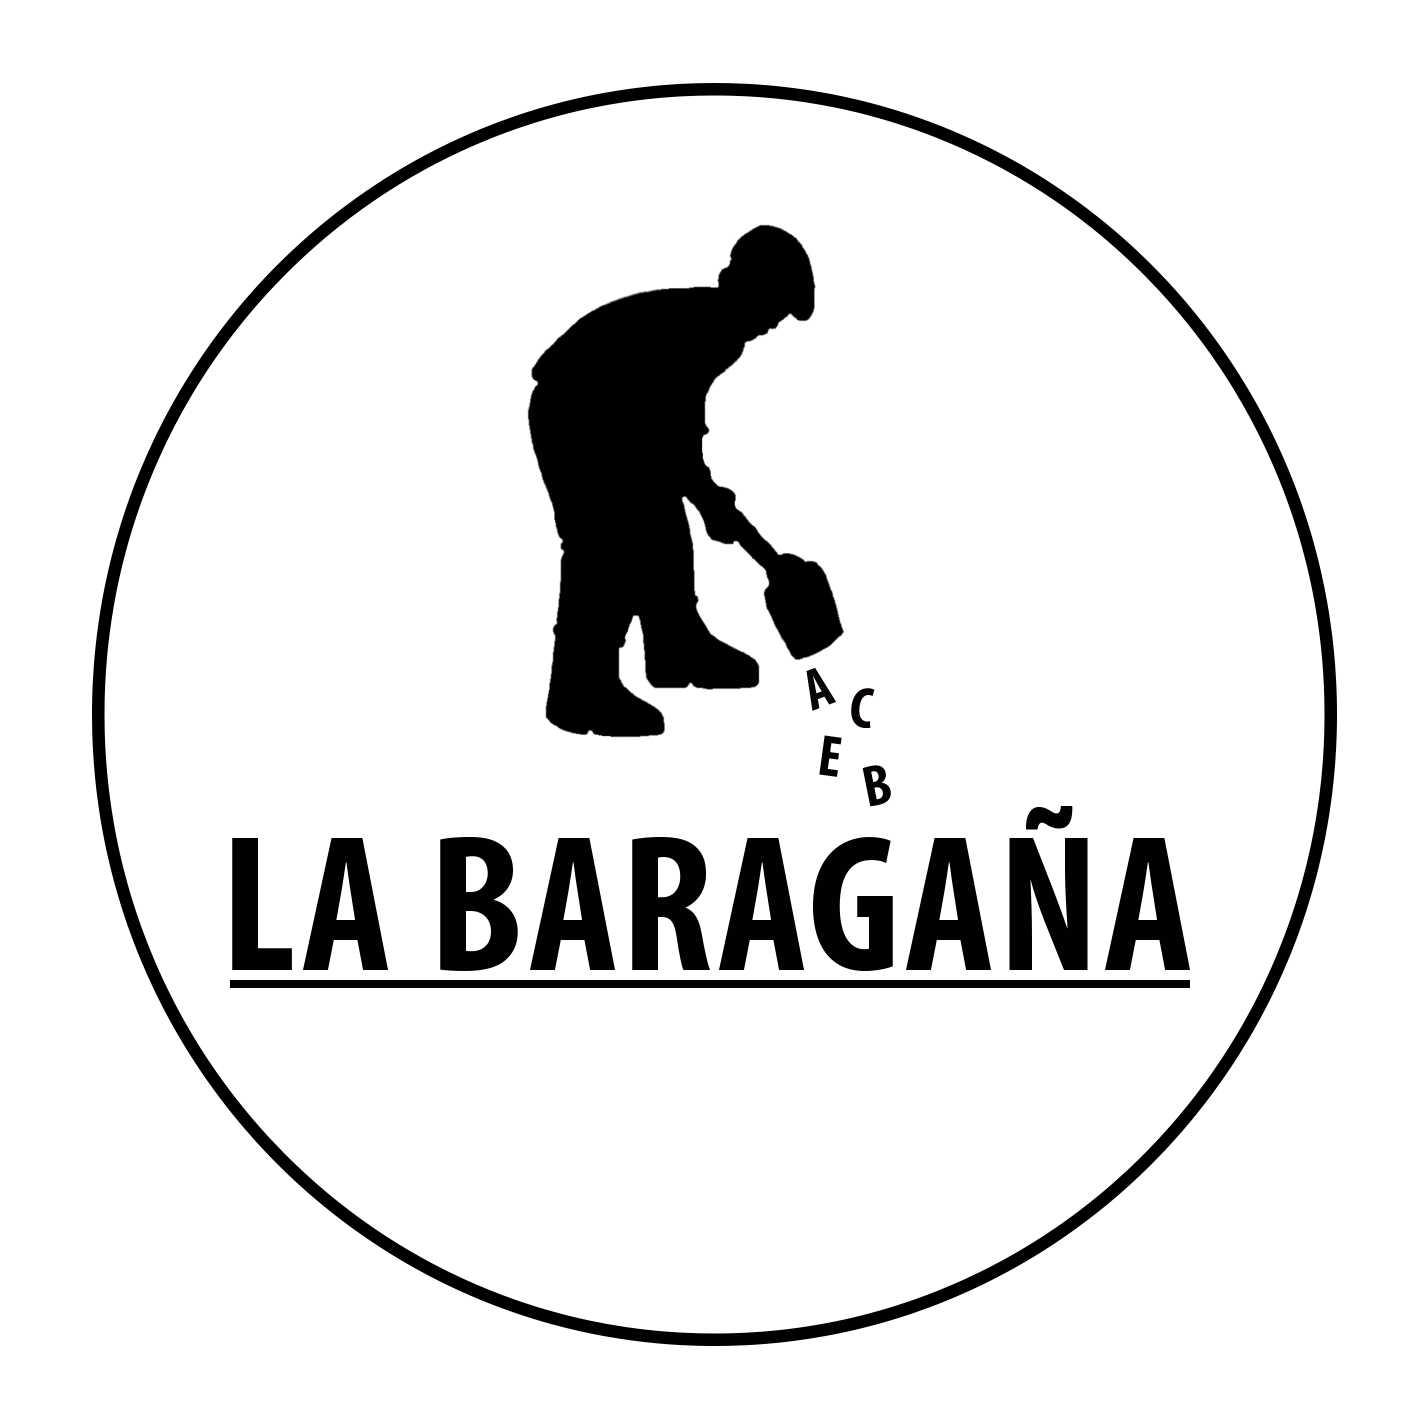
\includegraphics[width=0.5\textwidth]{../../../img/logo_back.png}
    \label{fig:logo}
\end{figure}

\end{document}
